%!TEX program = xelatex
% thesis.tex —— 本科毕业设计论文
% 题目：基于卫星雷达高度计近海回波波形仿真的海洋参数反演误差分析
%
% 基于 HUSTtex 模板（https://github.com/zfengg/HUSTtex/tree/master/HUSTthesis）修改
% 编译方式：XeLaTeX，编译两遍以生成目录
%
% 章节骨架说明（撰写阶段内部用，正式稿删除）：
%   - 红色批注 \hongzifuzhu{...} 标注“这一节写什么、放什么图/表”，成稿后删除
%   - 图源：../Echo_Simulation/output/ 与 ../Retracking/output/（已设 \graphicspath）
%   - 各章对应素材：
%       第3章  Echo_Simulation 各图（pm_surfaces / echo_wind_family / echo_speckle /
%              validation_u12 / thesis_style_waveforms / beach_fraction_scan /
%              reef_position_scan / island_position_scan / salinity_temperature）
%       第4章  Retracking fig1_calibration / fig4_hayne_models
%       第5章  Retracking fig2_speckle_error / fig3_nearshore_bias /
%              fig5_jason3_validation / fig6_mismatch_wind
%       第2章  原理示意图需新画（测高几何、脉冲有限足印、Brown 波形结构）
% ---------------------------------------------------------------------------- %

\documentclass[a4paper]{article}
% 10.5pt = 5 hao

% ---------------------------------- layout ---------------------------------- %
\usepackage[a4paper,top=2.5cm,bottom=2.5cm,left=3cm,right=3cm,% margins
			headheight=1.5cm,headsep=1.5em,
			footskip=2em,
			]{geometry}

% ------------------------------- math symbols ------------------------------- %
\usepackage{amsmath}
\usepackage{amsfonts}
\usepackage{amssymb}
\usepackage{mathrsfs}

%----------------------------------------------------------------%
%% linespace 行间距，段间距等等
\usepackage{setspace}
\renewcommand{\baselinestretch}{1.62}
\setlength{\baselineskip}{12pt}
\setlength\parskip{\baselineskip}
\setlength{\parindent}{0pt}

%----------------------------------------------------------------%
% fonts (style, color, size). 字体的大小，颜色，以及定义常用的字号
\usepackage{ctex}
% Chinese font
\usepackage{xeCJK}
\setCJKmainfont{FandolSong}
\setCJKsansfont{FandolSong}
\setCJKmonofont{FandolSong}
\setCJKfamilyfont{song}{FandolSong}
\newcommand{\song}{\CJKfamily{song}}
\setCJKfamilyfont{kai}{FandolKai}
\newcommand{\kai}{\CJKfamily{kai}}
\setCJKfamilyfont{hwzs}{FandolFang}
\newcommand{\hwzs}{\CJKfamily{hwzs}}
\setCJKfamilyfont{hei}{FandolHei}
\newcommand{\hei}{\CJKfamily{hei}}
% English font
\usepackage{fontspec}
\setmainfont{Times New Roman}
\setsansfont{Times New Roman}
\setmonofont{Times New Roman}
% font Color
\usepackage{xcolor}
\definecolor{MSBlue}{rgb}{.204,.353,.541}
\definecolor{MSLightBlue}{rgb}{.31,.506,.741}
% font Size
\newcommand{\xiaochuhao}{\fontsize{36pt}{\baselineskip}\selectfont}
\newcommand{\erhao}{\fontsize{21pt}{\baselineskip}\selectfont}
\newcommand{\xiaoerhao}{\fontsize{18pt}{\baselineskip}\selectfont}
\newcommand{\sanhao}{\fontsize{15.75pt}{\baselineskip}\selectfont}
\newcommand{\sihao}{\fontsize{14pt}{18pt}\selectfont}
\newcommand{\xiaosihao}{\fontsize{12pt}{18pt}\selectfont}
\newcommand{\wuhao}{\fontsize{10.5pt}{18pt}\selectfont}

% ---------------------------------------------------------------------------- %
%% header and footer 页眉，页脚
\usepackage{fancyhdr}
\newcommand{\headstyle}{
 \fancyhead[C]{ \hwzs\wuhao 华\hspace{0.5em}中\hspace{0.5em}科\hspace{0.5em}技\hspace{0.5em}大\hspace{0.5em}学\hspace{0.5em}毕\hspace{0.5em}业\hspace{0.5em}设\hspace{0.5em}计\hspace{0.5em}(论\hspace{0.5em}文)}
}
\newcommand{\footstyle}{\fancyfoot[C]{\wuhao\thepage}
 \fancyfoot[L]{\rule[5pt]{6.7cm}{0.4pt}}
 \fancyfoot[R]{\rule[5pt]{6.7cm}{0.4pt}}
}
\pagestyle{fancy}
\fancyhf{}
\headstyle
\footstyle
\fancypagestyle{main}{%
 \fancyhf{}
 \headstyle
 \footstyle
}
\renewcommand{\headrulewidth}{0.4pt}

% ---------------------------------------------------------------------------- %
% set the styles of sections at all levels
\usepackage{titlesec}
\usepackage{titletoc}
\titleformat{\section}{\centering\hei\bfseries\xiaoerhao}{\thesection}{1em}{}
\titleformat*{\subsection}{\raggedright\hei\bfseries\sihao}
\titleformat*{\subsubsection}{\raggedright\hei\bfseries\xiaosihao}
\titleformat{\paragraph}[hang]{\raggedright\hei\bfseries\xiaosihao}{\theparagraph}{1em}{}[]

\setcounter{tocdepth}{3}
\setcounter{secnumdepth}{3}

\newcommand{\sectionbreak}{\clearpage} % 每章从新的一页开始

% 正文内容样式命令：每节开始后调用 \seccontent
\newcommand\seccontent{
	\song
	\xiaosihao
    \setlength{\parindent}{2em}
    \setlength{\parskip}{0pt}
    }
\newcommand\tabcontent{
	\song
	\wuhao
    \setlength{\parindent}{2em}
    \setlength{\parskip}{0pt}
}

% ---------------------------------------------------------------------------- %
% for the caption and reference 图表及公式的编号规范
\usepackage{float}
\usepackage{caption}
\captionsetup[figure]{labelformat=default, labelsep=quad,name={图}}
\captionsetup[table]{labelformat=default,labelsep=quad,name={表}}
\renewcommand{\thefigure}{\ifnum \thesection>0 \thesection-\fi \arabic{figure}}
\renewcommand{\thetable}{\ifnum \thesection>0 \thesection-\fi \arabic{table}}
\DeclareCaptionFont{mylabelfont}{\hei\xiaosihao}
\captionsetup[figure]{font=mylabelfont}
\captionsetup[table]{font=mylabelfont}

\newcommand{\reffig}[1]{图 \ref{#1}}
\newcommand{\reftab}[1]{表 \ref{#1}}
\renewcommand\theequation{\arabic{section}-\arabic{equation}}

\usepackage{graphicx}
% 图源路径：直接引用三个代码模块的成品图
\graphicspath{{./}{../Echo_Simulation/output/}{../Retracking/output/}}
\usepackage{booktabs}
\usepackage{tabularx}
\usepackage{makecell}
\newcolumntype{L}{X}
\newcolumntype{C}{>{\centering \arraybackslash}X}
\newcolumntype{R}{>{\raggedright \arraybackslash}X}

% ---------------------------------------------------------------------------- %
% set the styles of counters 设置计数器
\makeatletter
\@addtoreset{footnote}{page}
\@addtoreset{figure}{section}
\@addtoreset{table}{section}
\@addtoreset{equation}{section}
\makeatother

% ---------------------------------------------------------------------------- %
% 目录
\usepackage{tocloft}
\renewcommand{\contentsname}{\centerline{ \hei\bfseries\xiaoerhao 目\hspace{2em}录}}
\titlecontents{section}[3em]{\song\xiaosihao\bfseries}{\contentslabel{3em}}{\hspace*{-3em}}{\normalfont\titlerule*[8pt]{.}\contentspage}
\titlecontents{subsection}[3em]{\song\xiaosihao}{\contentslabel{3em}}{\hspace*{-3em}}{\titlerule*[8pt]{.}\contentspage}
\titlecontents{subsubsection}[4em]{\song\xiaosihao}{\contentslabel{4em}}{\hspace*{-4em}}{\titlerule*[8pt]{.}\contentspage}

% ---------------------------------------------------------------------------- %
% reference and citation 参考文献
\usepackage[numbers]{natbib}
\renewcommand{\refname}{\centering\hei\xiaoerhao 参考文献}
\bibsep=0pt

% ---------------------------------------------------------------------------- %
% 设置声明页
\usepackage{wasysym}
\def\HUSTcheckedbox{$\Square\!\!\!\!\checkmark$}
\def\HUSTbox{$\Square$}
\newcommand{\statement}[2]{
	\def\yearofconfidentiality{\hspace{2em}}
    \def\HUSTconfidential{\HUSTbox}
	\def\HUSTnotconfidential{\HUSTcheckedbox}
	\ifnum #1<2
		\def\HUSTconfidential{\HUSTcheckedbox}
		\def\HUSTnotconfidential{\HUSTbox}
		\def\yearofconfidentiality{#2}
	\fi
	\clearpage
	\thispagestyle{main}
	\vspace*{1em}
	\seccontent
	\begin{center}
		\heiti \xiaoerhao \bfseries
		学位论文原创性声明
	\end{center}

    本人郑重声明：所呈交的论文是本人在导师的指导下独立进行研究所取得的研究成果。除了文中特别加以标注引用的内容外，本论文不包括任何其他个人或集体已经发表或撰写的成果作品。本人完全意识到本声明的法律后果由本人承担。

	\begin{flushright}
		作者签名：\hspace{6em} 年 \hspace{2em} 月 \hspace{2em} 日
	\end{flushright}
	\vspace{4em}

	\begin{center}
		\heiti \zihao{-2} \bfseries
		学位论文版权使用授权书
	\end{center}

    本学位论文作者完全了解学校有关保障、使用学位论文的规定，同意学校保留并向有关学位论文管理部门或机构送交论文的复印件和电子版，允许论文被查阅和借阅。本人授权省级优秀学士论文评选机构将本学位论文的全部或部分内容编入有关数据进行检索，可以采用影印、缩印或扫描等复制手段保存和汇编本学位论文。

    本学位论文属于 1、保密 \HUSTconfidential ，在 \yearofconfidentiality 年解密后适用本授权书。

		    \hspace{7em} 2、不保密 \HUSTnotconfidential \hspace{1em}
			。

			\hspace{7em} (请在以上相应方框内打``$\checkmark$'')


	\begin{flushright}
		作者签名：\hspace{6em} 年 \hspace{2em} 月 \hspace{2em} 日

	    导师签名：\hspace{6em} 年 \hspace{2em} 月 \hspace{2em} 日
	    \end{flushright}
	\clearpage
}
\newcommand{\makestatement}[2]{\statement{#1}{#2}}

% ---------------------------------------------------------------------------- %
% 定义中英文摘要和致谢环境
\newenvironment{cnabstract}[1]{
	\def \cnkeyword {#1}
	\clearpage
	\phantomsection
	\addcontentsline{toc}{section}{摘要}
	\vspace*{-20pt}
	\begin{center}
		\heiti \bfseries \xiaoerhao 摘 \hspace{2em} 要
	\end{center}
	\seccontent
}{
	\vspace{1em}
	\par\noindent {\hei\sihao \bfseries 关键词：} {\song\xiaosihao\cnkeyword}
}

\newenvironment{enabstract}[1]{
	\def \enkeyword {#1}
	\clearpage
	\phantomsection
	\addcontentsline{toc}{section}{Abstract}
	\vspace*{-20pt}
	\begin{center}
		\bfseries \xiaoerhao Abstract
	\end{center}
	\seccontent
}{
	\vspace{1em}
	\par\noindent {\sihao\bfseries Key Words: }\ {\song\xiaosihao\enkeyword}
	\clearpage
}

\newenvironment{thankpage}{
	\clearpage%
	\phantomsection%
	\addcontentsline{toc}{section}{致谢}%
	\section*{致\hspace{2em}谢}%
}{
	\clearpage
}

% ---------------------------------------------------------------------------- %
\usepackage{enumitem}
\setlist{noitemsep}
\usepackage{listings} % 代码（附录用）

% ---------------------------------------------------------------------------- %
\usepackage[bookmarks=true,colorlinks,linkcolor=black,citecolor=black,urlcolor=purple]{hyperref}

% ---------------------------------------------------------------------------- %
\usepackage{appendix}
\renewcommand{\appendixname}{附录}

% ---------------------------------------------------------------------------- %
% for the titlepage 标题页
\usepackage{titling}
\renewcommand{\maketitle}{
	\def\HUSTtitlelength{12em}
 	\begin{titlepage}
		\begin{center}
			\vspace*{0em}
			
\includegraphics[height=1.61cm]{HUSTlogo.eps}\\
%
			\vspace*{4em}
%
			{\xiaochuhao \hwzs \bfseries 本科生毕业设计[论文]}\\
%
			\vspace*{6em}
			{\erhao \hei \bfseries \thetitle}

			\vspace*{6em}
			{\sanhao \hwzs
				\renewcommand\arraystretch{2.7}
				\begin{tabular}{lc}
					\makebox[4em][s]{院 \hfill 系} &
					\underline{\makebox[\HUSTtitlelength]{\school}} \\
					\makebox[4em][s]{专业班级} &
					\underline{\makebox[\HUSTtitlelength]{\classnum}} \\
					\makebox[4em][s]{姓 \hfill 名} &
					\underline{\makebox[\HUSTtitlelength]{\theauthor}} \\
					\makebox[4em][s]{学 \hfill 号} &
					\underline{\makebox[\HUSTtitlelength]{\stunum}} \\
					\makebox[4em][s]{指导教师} &
					\underline{\makebox[\HUSTtitlelength]{\instructor}} \\
			  \end{tabular}
		    }

			\vspace{4em}
			{\sanhao \hwzs \thedate}

		\end{center}
	\end{titlepage}
}

% ------------------------------------ 标题页 ----------------------------------- %
\title{基于卫星雷达高度计近海回波波形仿真的海洋参数反演误差分析}
\def\school{电子信息与通信学院} % 院系
\def\classnum{电子信息工程} % 专业班级 TODO：补具体班号
\author{蒲奕帆} % 姓名
\def\stunum{U202213789}	% 学号
\def\instructor{田加胜} % 指导老师
\date{2026年5月6日} % TODO：按学校要求改为论文提交/答辩日期

% -------------------------------- quickinput -------------------------------- %
% 撰写阶段红字批注命令，成稿后删除所有调用
\newcommand{\hongzifuzhu}[1]{\textcolor{red}{\kai \wuhao(#1)}}

% ============================================================================ %
%                                  document                                    %
% ============================================================================ %
\begin{document}

\maketitle

% ------------------------------------ 声明页 ----------------------------------- %
\setcounter{page}{1}
\renewcommand{\thepage}{\Roman{page}}
\makestatement{2}{2019}

% ----------------------------------- 中文摘要 ----------------------------------- %
\begin{cnabstract}{卫星雷达高度计；波形仿真；近海；波形重跟踪；误差分析}
	\hongzifuzhu{中文摘要约 400--600 字，四段式：}
	\hongzifuzhu{（一）研究背景与意义（1--2 句）：卫星雷达高度计是全球海面高度/有效波高/海面风速观测的核心手段，近海回波受陆地带污染导致波形畸变，参数反演精度显著下降；}
	\hongzifuzhu{（二）本文做了什么：基于 PM 谱随机海面建立逐面元时域回波仿真模型（含 Brown 模型对照），实现近海沙滩/礁石/岛屿复合场景回波仿真；在此基础上实现阈值法、Brown 拟合与 Hayne 二阶模型三种重跟踪反演方法，构建“散斑随机误差—近海系统误差—模型失配误差”三层误差分析框架；}
	\hongzifuzhu{（三）主要结果（给数字）：如礁石位于天底点时 SSH 偏差 +40 cm、岛屿 +78 cm；散斑误差随平均门数按 1/sqrt(N) 收敛；拟合残差 RMS 可作波形质量判据并被 Jason-3 实测数据印证（近海 10.9\% vs 开阔海 8.1\%）等；}
	\hongzifuzhu{（四）结论与意义一句话。关键词 3--5 个。}
\end{cnabstract}

% ----------------------------------- 英文摘要 ----------------------------------- %
\begin{enabstract}{satellite radar altimeter; waveform simulation; coastal zone; waveform retracking; error analysis}
	\hongzifuzhu{英文摘要与中文摘要内容一一对应，写完中文后翻译润色。}
\end{enabstract}

% ------------------------------------ 目录 ------------------------------------ %
% 注：不用 \tableofcontents —— 它经 \section* 排标题，会触发 titlesec 的
% \sectionbreak（\clearpage），在目录前弹出一页空白页；此处手工排标题后
% 直接 \@starttoc 读目录，条目间留少量胶水使其可正常跨页。
\begingroup
\setcounter{tocdepth}{2} % 目录显示到二级标题
{\centering {\hei\bfseries\xiaoerhao 目\hspace{2em}录}\par}
\vspace{0.5em}
\makeatletter
\parskip=2pt plus 1pt minus 1pt
\@starttoc{toc}
\makeatother
\endgroup
\thispagestyle{main}

\clearpage
\setcounter{page}{1}
\renewcommand{\thepage}{\arabic{page}}

% ============================================================================ %
%                                  主体内容                                     %
% ============================================================================ %
\seccontent

% ---------------------------------------------------------------------------- %
\section{绪论}
\label{chap:intro}

\subsection{研究背景与意义}
\label{sec:background}
\hongzifuzhu{写什么：卫星雷达高度计对全球海洋观测的价值（海面高度→大尺度海洋环流/海平面上升，有效波高→波浪预报，$\sigma^0$→风速）；测高卫星系列一句话带过（Topex/Poseidon—Jason—Sentinel-6）；引出问题——近海（<10 km）区域回波受陆地污染、波形畸变，标准产品精度下降，而近海恰是航运/风暴潮/ coastal 灾害重点区。落点：本文通过“仿真+反演+误差分析”闭环定量回答“近海回波畸变如何映射为参数反演误差”。}

\subsection{国内外研究现状}
\label{sec:related}
\hongzifuzhu{写什么（三块，各 3--5 段，要有引文）：}
\hongzifuzhu{（一）测高卫星与数据处理的发展：Jason-1/2/3、Sentinel-6 MF，SGDR/GDR 产品与 MLE3/MLE4 重跟踪；}
\hongzifuzhu{（二）海面回波仿真方法：Brown（1977）卷积模型、Hayne（1980）二阶解析模型、逐面元时域/频域仿真、海面谱模型（PM 谱、Eluhihb 一维谱等）；}
\hongzifuzhu{（三）波形重跟踪与近海处理：OCOG/阈值法、Beta5/9 拟合、物理法（Brown/Hayne 拟合）、近海专用算法（如 ALES、 coastal retracking）；国内近海高度计研究简述。}
\hongzifuzhu{引用的参考文献/ 需要整理成 bib 条目。}

\subsection{本文主要工作与章节安排}
\label{sec:outline}
\hongzifuzhu{写什么：逐条列出本文四项工作（海面与回波仿真、近海场景扩展、三种重跟踪反演实现、三层误差分析与 Jason-3 实测验证），然后一段话给出各章内容安排。}

\sectionbreak

% ---------------------------------------------------------------------------- %
\section{卫星雷达高度计海洋回波测量原理}
\label{chap:principle}

\subsection{高度计测距与脉冲有限工作体制}
\label{sec:altimeter-principle}
\hongzifuzhu{写什么：测高基本几何（卫星到海面距离+轨道→SSH）；脉冲有限（pulse-limited）体制足印随时间扩大的过程；Jason-3 关键系统参数（ Ku 波段 13.575 GHz、轨道高度 1336 km、带宽 320 MHz、104 距离门×3.125 ns）。}
\hongzifuzhu{建议配图：测高几何示意图、脉冲有限足印示意图（需新画，Visio/TikZ）。}

\subsection{海面电磁散射与回波功率}
\label{sec:scatter}
\hongzifuzhu{写什么：几何光学（GO）近似下准镜面散射，Cox-Munk 斜率概率密度与 $\sigma^0$ 随风速的关系；雷达方程作用于扩散足印内各面元。公式：本文式(4.5)-(4.10) 对应的散射理论。}

\subsection{Brown 平均回波模型与 Hayne 二阶模型}
\label{sec:brown-hayne}
\hongzifuzhu{写什么：Brown 三重卷积模型（平坦海面冲激响应 $\ast$ 波高概率密度 $\ast$ 点目标响应）各项物理含义与波形三段结构（热噪声区/上升沿/平顶）；Hayne 二阶模型解析式及误指向角 ξ 项；波形关键参数（amplitude、半功率点 $t_0$、前沿斜率→$\sigma_h$）与海洋参数的对应。}
\hongzifuzhu{可复用 Echo\_Simulation/output/echo\_wind\_family.png 作为波形结构示意（或据此重绘标注版）。}

\subsection{海水介电常数与菲涅尔反射率}
\label{sec:dielectric}
\hongzifuzhu{写什么：Debye 介电模型（盐度/温度→复介电常数→垂直入射菲涅尔反射率 ρ）；给出 Ku 波段锚点 ε=(47.08, 39.07)、ρ=0.6173；说明回波平台功率与 ρ 的关系。}

\subsection{近海回波的特殊性}
\label{sec:coastal-specific}
\hongzifuzhu{写什么：近海波形污染的三种典型机制——足印部分触陆（陆地带回波叠加）、浅水海况与开阔海差异、地形（滩涂/礁石/岛屿）造成的提前回波；由此引出“标准重跟踪在近海失效”的问题。}
\hongzifuzhu{建议配图：可用 Jason-3 c603p147 近海实测波形堆叠图作直观例子（Data\_Reading 的 nearshore\_stack 成品图，或 Retracking fig5）。}

\sectionbreak

% ---------------------------------------------------------------------------- %
\section{基于 PM 谱海面的近海回波波形仿真}
\label{chap:simulation}

本章建立卫星雷达高度计海面回波的时域仿真模型并给出仿真结果。第 \ref{sec:sim-framework} 节给出总体框架与系统参数；第 \ref{sec:pm-surface} 节给出 PM 方向谱随机海面的生成方法与有限网格口径；第 \ref{sec:facetsim} 节建立逐面元时域回波模型；第 \ref{sec:sim-validation} 节以 Brown 模型为基准验证仿真链路的正确性；第 \ref{sec:coastal-sim} 节将近海陆地要素引入海面，仿真沙滩、礁石、岛屿三类复合场景的回波畸变，并分析海水盐度与温度的影响。

\subsection{仿真总体框架}
\label{sec:sim-framework}

本文以 Jason-3 卫星雷达高度计为仿真对象。其 Ku 波段（13.575 GHz）天线 3 dB 波束宽度为 2.2$^\circ$，对应轨道高度（1336 km）上天底点 $-3$ dB 足印半径约 25.7 km；而压缩后脉冲宽度对应的空间尺度仅约 0.47 m，远小于波束足印，属于典型的脉冲有限（pulse-limited）体制。脉冲有限体制下，平均回波由“脉冲受限环”自天底点随时间向外扩张的响应主导，这正是 Brown 模型\cite{brown1977}描述的物理图像（详见第 2 章）。

仿真按如下四个环节进行，各环节的数学模型分别在 3.2 与 3.3 节给出：
\begin{enumerate}
	\item \textbf{海面生成}：由二维 PM 方向谱经 FFT 线性滤波生成随机海面高度场 $\eta(x, y)$；
	\item \textbf{逐面元散射}：将海面离散为边长 $\mathrm{d}x$ 的方形面元，按几何光学（GO）近似计算面元后向散射系数 $\sigma^0$，并由雷达方程计算其回波功率贡献；
	\item \textbf{延迟分箱}：按每个面元的双程延迟 $\tau = 2R/c$ 将其功率累加到精细时间网格；
	\item \textbf{系统响应}：与雷达点目标响应卷积并按距离门积分，得到 104 门回波波形；对 $M$ 个独立随机海面实现重复上述过程并取系综平均。
\end{enumerate}

仿真采用两尺度（two-scale）口径：PM 网格（$\mathrm{d}x = 15.625$ m，可分辨的最短波长约 31.2 m）显式承载长重力波的波高分布与延迟分布；短波对 $\sigma^0$ 的贡献由包含全部波段的 Cox--Munk 斜率统计量承载，不在网格中显式生成。该口径的适用范围与方差补偿见 \ref{sec:pm-surface} 节。

仿真系统参数与参考论文\cite{refpaper}保持一致，列于\reftab{tab:params}；距离门配置与 Jason-3 SGDR Ku 波段一致（104 门、门间隔 3.125 ns）。海面域边长取 $L = 32$ km：采样窗末端（$+272$ ns）脉冲受限环半径约 10.4 km，由 $\tau \approx r^{2}/(cH)$ 估算，32 km 域完整容纳窗口内全部环带贡献，空间截断不损失窗口内回波能量。

\begin{table}[htpb]
	\centering
	\caption{雷达高度计仿真系统参数}
	\label{tab:params}
	\song\wuhao
	\begin{tabular}{lcc}
		\toprule
		参数 & 符号 & 数值 \\
		\hline
		轨道高度 & $H$ & 1336 km \\
		Ku 波段中心频率 & $f$ & 13.575 GHz \\
		雷达波长 & $\lambda$ & 2.21 cm \\
		峰值发射功率 & $P_t$ & 50 W \\
		天线 3 dB 波束宽度 & & $2.2^\circ$ \\
		采样率（带宽） & $B$ & 320 MHz \\
		距离门数 & & 104 \\
		距离门间隔 & & 3.125 ns（0.469 m） \\
		采样窗（相对平均海平面双程延迟） & & $-50$ ~ $+272$ ns \\
		海水相对介电常数 & $\varepsilon_s$ & $47.08 + 39.07\,\mathrm{j}$ \\
		法向菲涅尔反射率 & $\rho$ & 0.6173 \\
		\bottomrule
	\end{tabular}
\end{table}

\hongzifuzhu{TODO：此处可补一幅仿真流程框图（海面生成→散射→分箱→系统响应→系综平均），用 Visio/TikZ 画。}

\subsection{PM 方向谱随机海面的生成}
\label{sec:pm-surface}

\subsubsection{PM 谱及其参数}

充分发展风浪采用 Pierson--Moskowitz（PM）谱\cite{pm1964}描述。以波数 $k$ 表示的一维 PM 谱为
\begin{equation}
	W(k) = \frac{\alpha}{2k^{3}} \exp\!\left( -\frac{\beta g^{2}}{k^{2} U_{19.5}^{4}} \right), \qquad k > 0
	\label{eq:pm1d}
\end{equation}
式中 $\alpha = 8.10 \times 10^{-3}$ 与 $\beta = 0.74$ 为经验常数，$g$ 为重力加速度，$U_{19.5}$ 为海面以上 19.5 m 高度风速。对式 \eqref{eq:pm1d} 积分可得海面均方根高度及有效波高（SWH）
\begin{equation}
	\sigma_h = \left( \frac{\alpha U_{19.5}^{4}}{4 \beta g^{2}} \right)^{1/2}, \qquad \mathrm{SWH} = 4 \sigma_h
	\label{eq:swh}
\end{equation}
不同参考高度的风速换算采用文献\cite{refpaper}的口径：
\begin{equation}
	U_{19.5} = U_{10} \left( 1 + \frac{\sqrt{5 \times 10^{-4}\, U_{10}^{1/2}}}{0.4} \ln 10 \right)
	\label{eq:u19}
\end{equation}
式中 $U_{10}$ 为 10 m 高度风速。

二维方向谱在一维谱基础上引入 $\cos^{2}$ 型方向展宽：
\begin{equation}
	W(k_x, k_y) = \frac{\alpha}{2 K^{4}} \exp\!\left( -\frac{\beta g^{2}}{K^{2} U_{19.5}^{4}} \right) \frac{\cos^{2}(\theta_k - \phi_v)}{\pi}
	\label{eq:pm2d}
\end{equation}
式中 $K = \sqrt{k_x^{2} + k_y^{2}}$ 为波数模，$\theta_k$ 为波数方向角，$\phi_v$ 为风向。需要说明，$\cos^{2}/\pi$ 展宽因子在全平面内积分为 $1/2$，即该方向谱仅承载一维谱一半的方差；此差异并入下文方差解析比例一并补偿，不单独修正。

\subsubsection{FFT 线性滤波法}

随机海面采用谱域线性滤波法\cite{thorsos1990}生成：在离散波数网格上，对单位方差复高斯白噪声谱 $\hat\Gamma$ 施加谱幅滤波后作逆傅里叶变换并取实部，
\begin{equation}
\begin{aligned}
	\eta(x, y) &= 2\, \mathrm{Re} \left\{ \mathrm{IFFT}_2 \left[ H_F(k_x, k_y)\, \hat\Gamma(k_x, k_y) \right] \right\} \\
	H_F(k_x, k_y) &= \frac{N^{2}}{\sqrt{2}} \sqrt{W(k_x, k_y)\, \Delta k_x \Delta k_y}
\end{aligned}
\label{eq:fft}
\end{equation}
式中 $N$ 为每边采样点数，$\Delta k_x = \Delta k_y = 2\pi/L$ 为波数分辨率；因子 $N^{2}/\sqrt{2}$ 与“取实部加倍”共同保证 $\eta$ 的谱密度收敛到 $W$。本文实现与第 2 章海面仿真的 MATLAB 模块（FFT 线性滤波法）保持一致。

\subsubsection{有限网格口径与方差补偿}

有限海面域只能表示 $k_{\min} = 2\pi/L$ 至 $k_{\max} = \pi/\mathrm{d}x$ 范围内的波数。本文取 $L = 32$ km、$N = 2048$（$\mathrm{d}x = 15.625$ m），对应 $k_{\max} = 0.201$ rad/m。网格可解析的谱方差占比（capture）为
\begin{equation}
	\gamma_{\mathrm{cap}} = \left( \frac{\sigma_{\mathrm{grid}}}{\sigma_h} \right)^{2} \approx \exp\!\left( -\frac{\beta g^{2}}{k_{\max}^{2} U_{19.5}^{4}} \right)
	\label{eq:capture}
\end{equation}
式中 $\sigma_{\mathrm{grid}} = \left( \sum W \Delta k_x \Delta k_y \right)^{1/2}$ 为本网格谱期望的均方根高度。PM 谱是宽谱，风速越低能量越集中于短重力波，$\gamma_{\mathrm{cap}}$ 随之骤降：$U_{19.5} = 8/12/16$ m/s 时分别约为 65.0\%/91.9\%/97.3\%。

为使波高统计不受网格截断影响，本文将生成的海面高度场归一化到完整 PM 理论值 $\sigma_h$（式 \eqref{eq:swh}），以补偿未解析波段与方向谱展宽损失的方差；其代价是已解析长波的斜率被同步放大。在默认的几何入射角口径下（见 \ref{sec:facetsim} 节）斜率不参与散射调制，该代价无影响；仅在启用长波倾斜调制的诊断运行（第 \ref{chap:error} 章）中需要计入。当 $U_{19.5} < 6$ m/s 时 $\gamma_{\mathrm{cap}}$ 过低，归一化放大失真显著，该口径不再适用，需改用显式两尺度分解（见第 6 章展望）。

\reftab{tab:seastates} 给出本文采用的三档海况及其关键参数；\reffig{fig:pm} 为三档风速下生成的海面样例。天底 $\sigma^0(0) = \rho / (2 \sqrt{\sigma_u^{2} \sigma_c^{2}})$ 随风速增大而下降（13.22/12.51/11.90 dB），是高度计风速测量的物理基础（见 \ref{sec:facetsim} 节）。

\begin{table}[htpb]
	\centering
	\caption{仿真海况组及其关键参数}
	\label{tab:seastates}
	\song\wuhao
	\begin{tabular}{cccccc}
		\toprule
		$U_{19.5}$ (m/s) & $U_{10}$ (m/s) & SWH (m) & $\sigma_h$ (m) & $\sigma^0(0)$ (dB) & $\gamma_{\mathrm{cap}}$ \\
		\hline
		8  & 6.63  & 1.365 & 0.3413 & 13.22 & 65.0\% \\
		12 & 9.78  & 3.071 & 0.7679 & 12.51 & 91.9\% \\
		16 & 12.86 & 5.460 & 1.3651 & 11.90 & 97.3\% \\
		\bottomrule
	\end{tabular}
\end{table}

\begin{figure}[H]
	\centering
	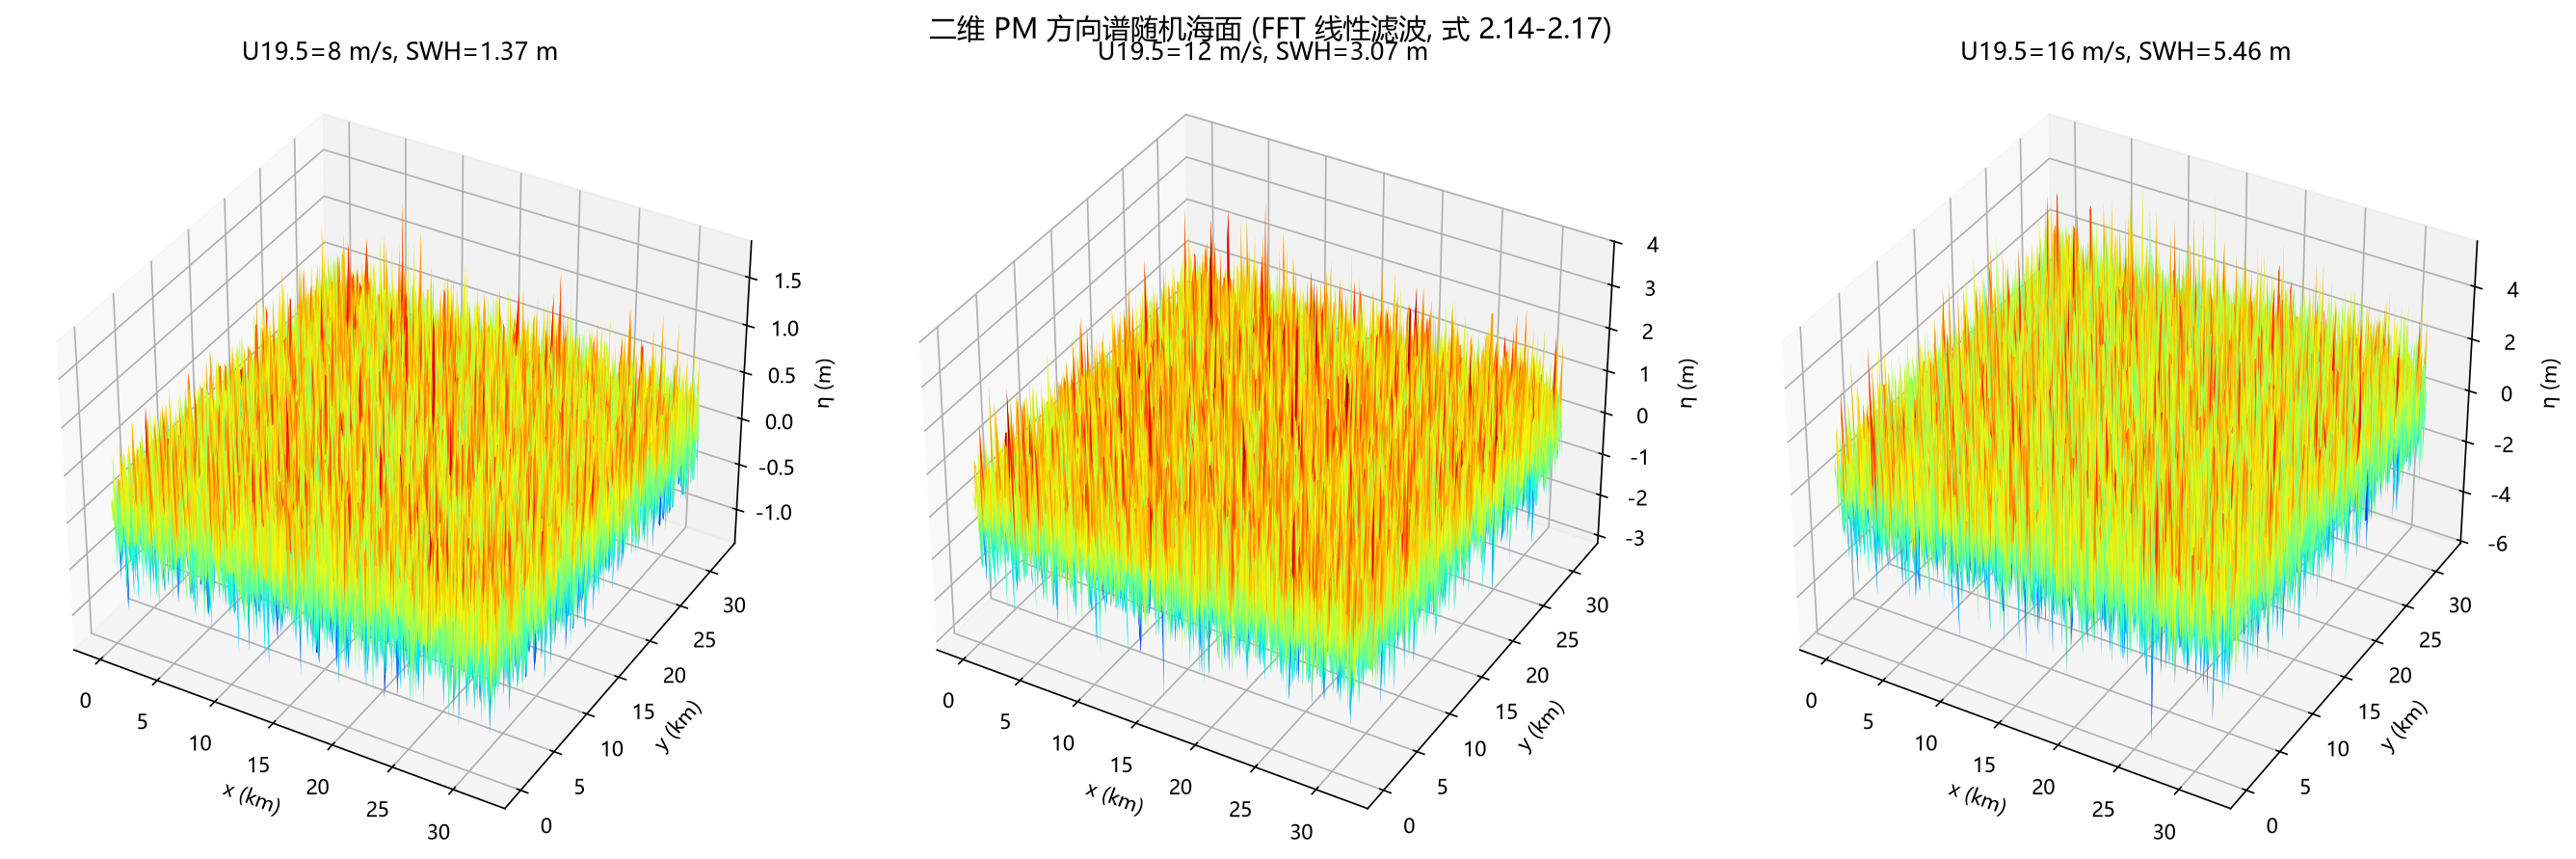
\includegraphics[width=0.98\textwidth]{pm_surfaces.png}
	\caption{三档风速下的二维 PM 方向谱随机海面样例（32 km 域，125 m 间隔抽样显示）}
	\label{fig:pm}
\end{figure}

\subsection{逐面元时域回波仿真方法}
\label{sec:facetsim}

\subsubsection{面元几何与散射模型}

对位于 $(x, y)$、高度为 $\eta$ 的面元，其到天底指向雷达的斜距、双程延迟与几何入射角为（对应文献\cite{refpaper}式(4.1)）
\begin{equation}
	R = \sqrt{x^{2} + y^{2} + (H - \eta)^{2}}, \qquad \tau = \frac{2R}{c}, \qquad \theta = \arctan \frac{\sqrt{x^{2} + y^{2}}}{H}
	\label{eq:geom}
\end{equation}
天线采用高斯功率方向图
\begin{equation}
	G(\theta) = \exp\!\left( -\frac{\theta^{2}}{2 \sigma_\theta^{2}} \right)
	\label{eq:gain}
\end{equation}
$\sigma_\theta$ 由半功率角确定：$\theta$ 等于半波束宽度 $1.1^\circ$ 时 $G$ 降至 $1/2$，解得 $\sigma_\theta = 0.934^\circ$。

面元后向散射采用几何光学（GO）近似与各向异性 Cox--Munk 斜率概率密度\cite{coxmunk1954}：
\begin{equation}
	\sigma^0(\theta, \phi) = \frac{\rho\, \pi}{\cos^{4} \theta}\, p\!\left( \tan\theta, 0 \right), \qquad p = \frac{1}{2 \pi \sqrt{\sigma_u^{2} \sigma_c^{2}}} \exp\!\left( -\frac{\tan^{2} \theta}{v} \right)
	\label{eq:sigma0}
\end{equation}
\begin{equation}
	\frac{1}{v} = \frac{1}{2} \left( \frac{\cos^{2}(\phi - \phi_v)}{\sigma_u^{2}} + \frac{\sin^{2}(\phi - \phi_v)}{\sigma_c^{2}} \right)
	\label{eq:vdef}
\end{equation}
式中 $\phi$ 为面元方位角，$\sigma_u^{2}$、$\sigma_c^{2}$ 分别为顺风向与交叉风向斜率方差，取 Cox--Munk 型随风速线性变化的经验关系（对应文献\cite{refpaper}式(4.9)、(4.10)）：
\begin{equation}
	\sigma_u^{2} = 0.00078545\, U_{19.5} + 0.0092407, \qquad \sigma_c^{2} = 0.00052799\, U_{19.5} + 0.0097295
	\label{eq:slopevar}
\end{equation}

两尺度口径在此体现为：式 \eqref{eq:slopevar} 的斜率统计包含全部波段的贡献（短波不可解析，由统计量承载），而波高分布与延迟分布仅由 PM 长波海面承载。面元散射按几何入射角计算，即长波倾斜不调制 $\sigma^0$——这与 Brown 模型的假设严格一致，便于 \ref{sec:sim-validation} 节的同口径对照；长波倾斜的调制作为二阶效应在第 \ref{chap:error} 章单独讨论。

\subsubsection{雷达方程与延迟分箱}

每个面元的回波功率贡献由雷达方程给出（对应文献\cite{refpaper}式(4.1)--(4.4)）：
\begin{equation}
	\mathrm{d} P(\tau) = \frac{\lambda^{2} P_t\, G^{2}(\theta)\, \sigma^0(\theta, \phi)\, \mathrm{d}S}{(4 \pi)^{3} R^{4}}
	\label{eq:radar}
\end{equation}
式中 $\mathrm{d}S = \mathrm{d}x^{2}$ 为面元面积。将全部面元的贡献按双程延迟 $\tau$ 分箱累加到精细时间网格（每距离门细分为 $q = 4$ 格，精细间隔 0.781 ns），得到回波功率密度；再与雷达理想点目标响应
\begin{equation}
	S_r(\tau) = \left( \frac{\sin(\pi B \tau)}{\pi B \tau} \right)^{2}
	\label{eq:ptr}
\end{equation}
卷积（$B = 320$ MHz），并在每个距离门内积分，得到 104 门回波波形。点目标响应描述压缩后脉冲的时间展宽，决定了波形上升沿的最小陡峭度。

\subsubsection{散斑与系综平均}

单个随机海面实现的回波波形呈现剧烈的随机起伏（散斑），这是大量面元散射随机叠加的必然结果，也是实际高度计 20 Hz 波形散斑的物理来源。对 $M = 24$ 个独立海面实现取系综平均后，波形收敛到光滑的平均回波，如\reffig{fig:speckle} 所示；散斑导致的随机反演误差在第 \ref{chap:error} 章定量分析。

\reffig{fig:windfamily} 给出三档海况的系综平均波形族（实线）与 Brown 数值模型（虚线，见 \ref{sec:sim-validation} 节）：SWH 越大上升沿越缓（前沿 10\%--90\% 宽度随 SWH 展宽），$\sigma^0$ 随风速下降使平台功率降低，与第 2 章波形三段结构的理论预期一致。\reffig{fig:thesisstyle} 为单次实现的逐门折线呈现（$U_{19.5} = 4/8/12$ m/s），呈现方式与文献\cite{refpaper}图 4.3 一致，直观展示实际接收波形的散斑形态。

\begin{figure}[H]
	\centering
	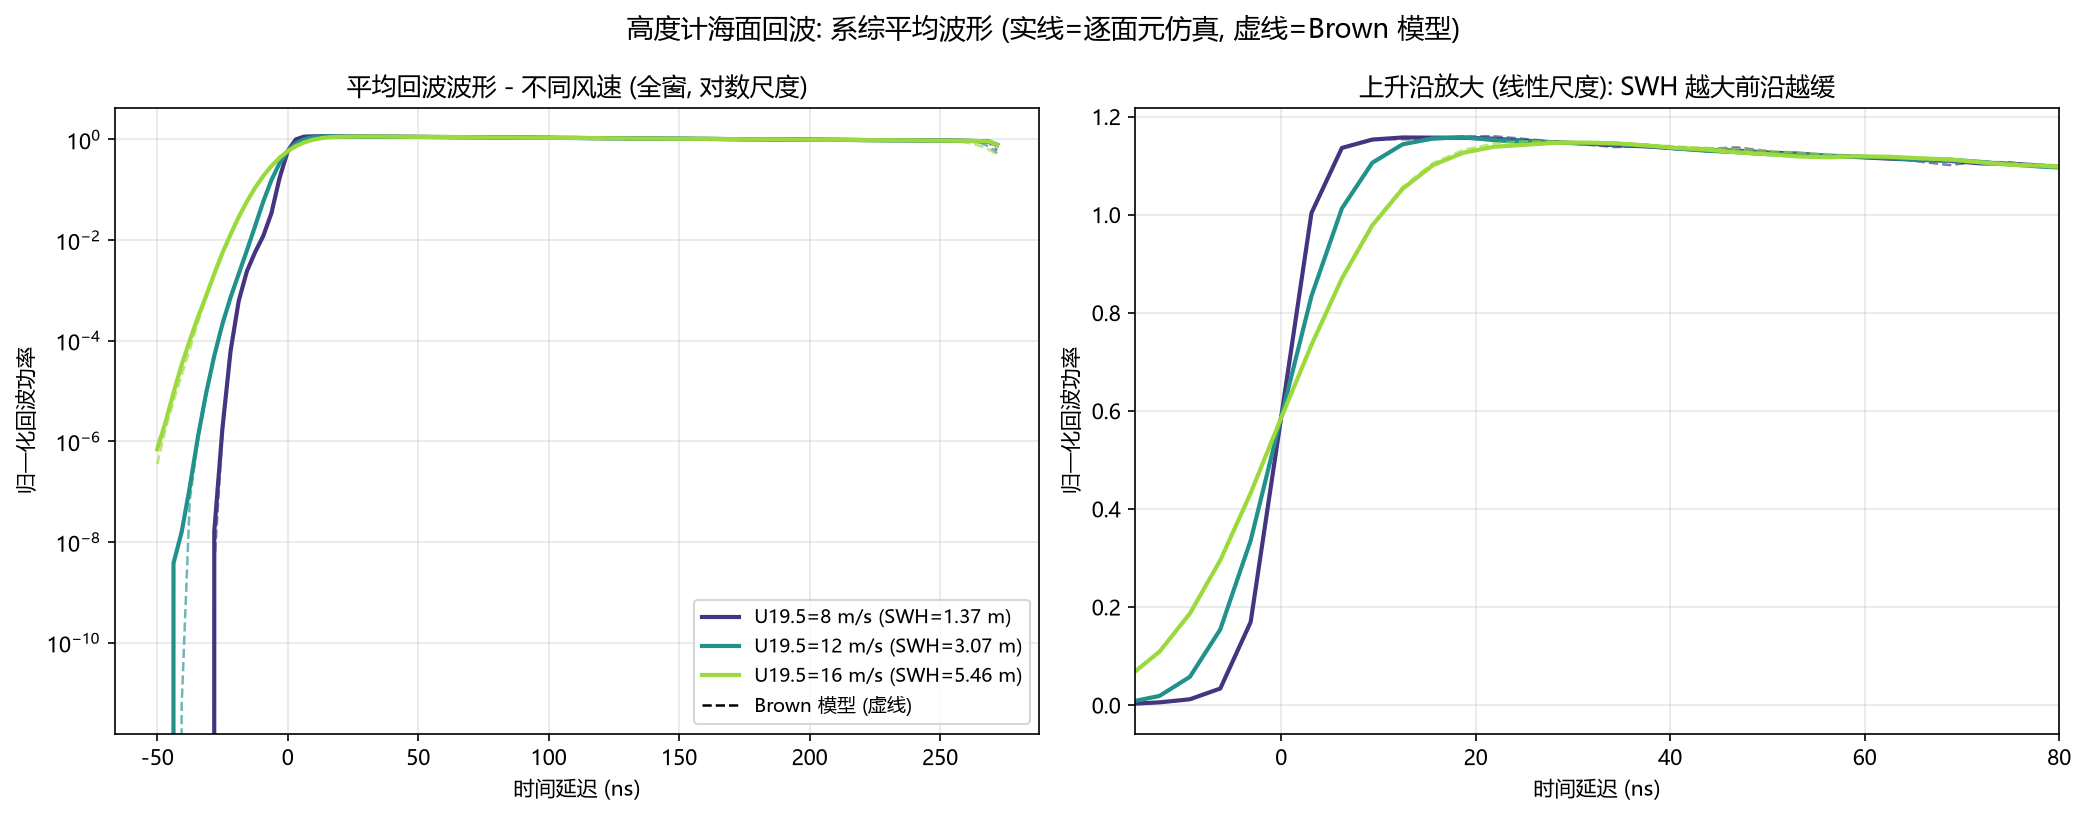
\includegraphics[width=\textwidth]{echo_wind_family.png}
	\caption{三档海况的系综平均回波波形族（实线：逐面元仿真，$M = 24$；虚线：Brown 数值模型）。左：全窗对数尺度；右：上升沿线性放大}
	\label{fig:windfamily}
\end{figure}

\begin{figure}[H]
	\centering
	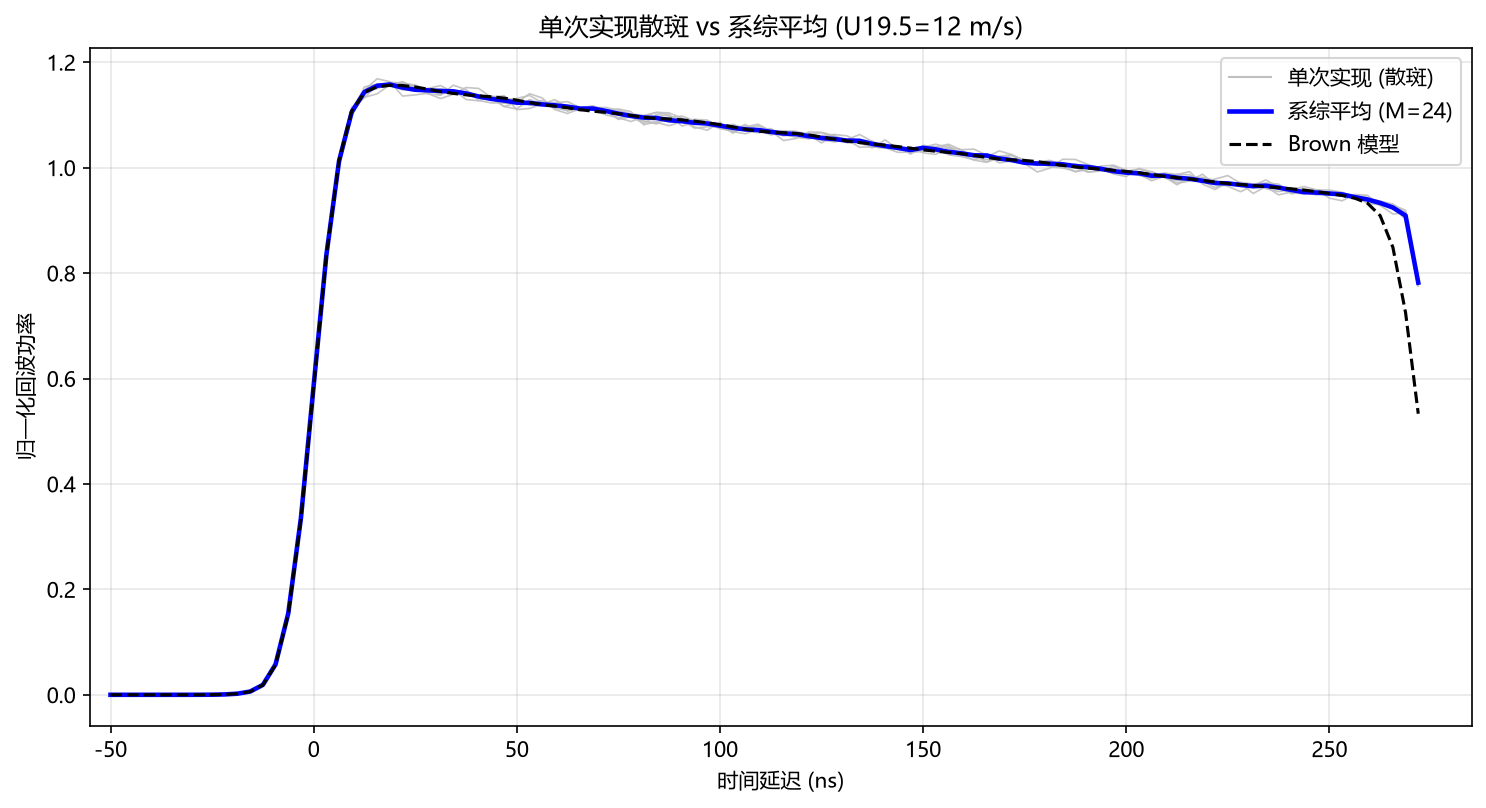
\includegraphics[width=0.85\textwidth]{echo_speckle.png}
	\caption{单次实现的散斑波形与系综平均（$U_{19.5} = 12$ m/s，$M = 24$）}
	\label{fig:speckle}
\end{figure}

\begin{figure}[H]
	\centering
	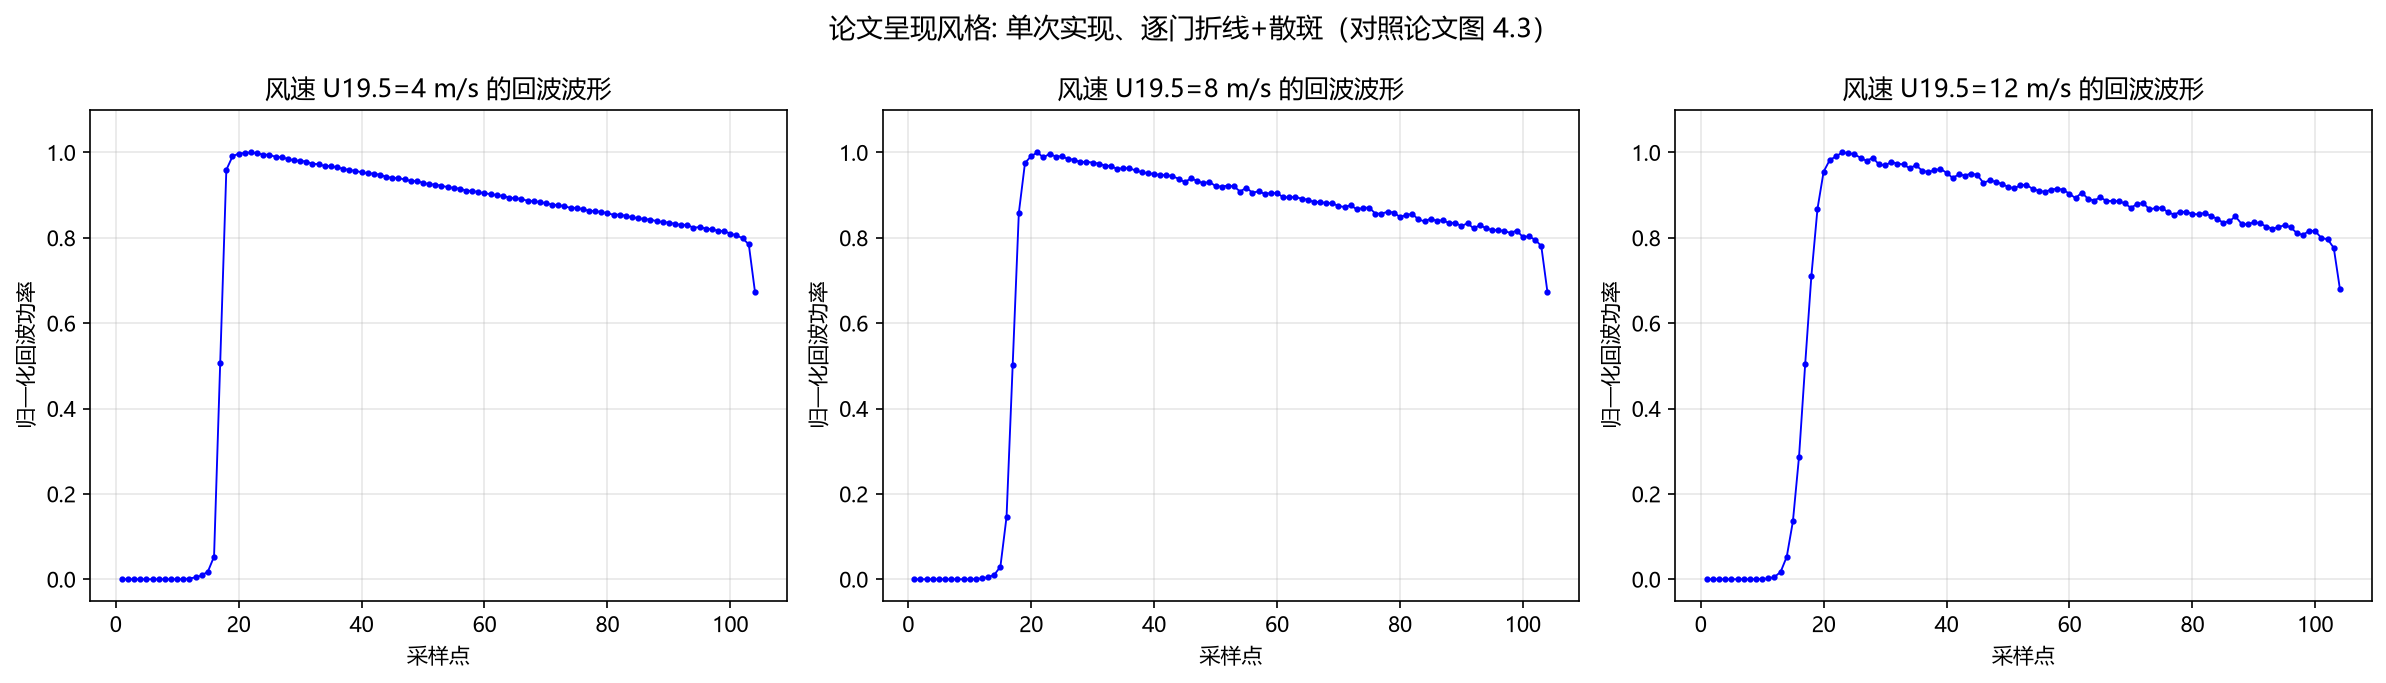
\includegraphics[width=\textwidth]{thesis_style_waveforms.png}
	\caption{单次实现回波的逐门折线呈现（$U_{19.5} = 4/8/12$ m/s），呈现方式与文献\cite{refpaper}图 4.3 一致}
	\label{fig:thesisstyle}
\end{figure}

\subsection{仿真结果的 Brown 模型对照验证}
\label{sec:sim-validation}

Brown 平均回波模型\cite{brown1977}将平均回波表示为三个物理因子的卷积：
\begin{equation}
	W(t) = P_{\mathrm{FS}}(t) \ast q_s(t) \ast S_r(t)
	\label{eq:brown}
\end{equation}
式中 $P_{\mathrm{FS}}$ 为平坦海面冲激响应，$q_s$ 为海面波高概率密度（本文取高斯形式，标准差 $\sigma_\tau = 2 \sigma_h / c$，偏度 $\lambda_s = 0$），$S_r$ 为点目标响应（式 \eqref{eq:ptr}）。Hayne\cite{hayne1980}给出了包含误指向角与偏度修正的二阶解析展开，其零阶形式即式 \eqref{eq:brown}，第 2 章已作详细讨论。

本文采用“同口径数值对照”的验证策略：$P_{\mathrm{FS}}$ 不使用解析式，而用与逐面元仿真完全相同的代码路径计算——海面高度取零的平面、同一几何、增益、散射模型、分箱方式与空间截断。这样，两种方法在所有数值口径上严格一致，差异只来自“随机起伏海面与平面”本身，系综平均的逐面元仿真应收敛到 Brown 数值模型。相比与解析式的比较，这是一条口径更干净的正确性检验。

\reffig{fig:val} 给出 $U_{19.5} = 12$ m/s（SWH $= 3.07$ m）的对照结果。以平台区功率归一化后：前沿区（$-20$ ~ $+80$ ns）相对偏差 RMS 为 0.74\%，平台功率比（仿真/Brown）为 1.0002；三档海况的前沿区偏差 RMS 均不超过 0.8\%，平台功率比偏差不超过 0.3\%。偏差集中在波形端部——前缘之前的“提前回波”与远尾（$> 180$ ns，5\%--14\% 且随风速增大）——机理是归一化 PM 长波海面的波高概率密度在端部偏离高斯假设，其中前缘前提前回波偏强（约 1\%）正是第 \ref{chap:error} 章模型失配分析中 SWH 系统性低估 10\%--16\% 的原因（见 \ref{sec:mismatch-error} 节）。反演关注的平台区与前沿区一致性在 1\% 以内，仿真链路的正确性得到验证。

\begin{figure}[H]
	\centering
	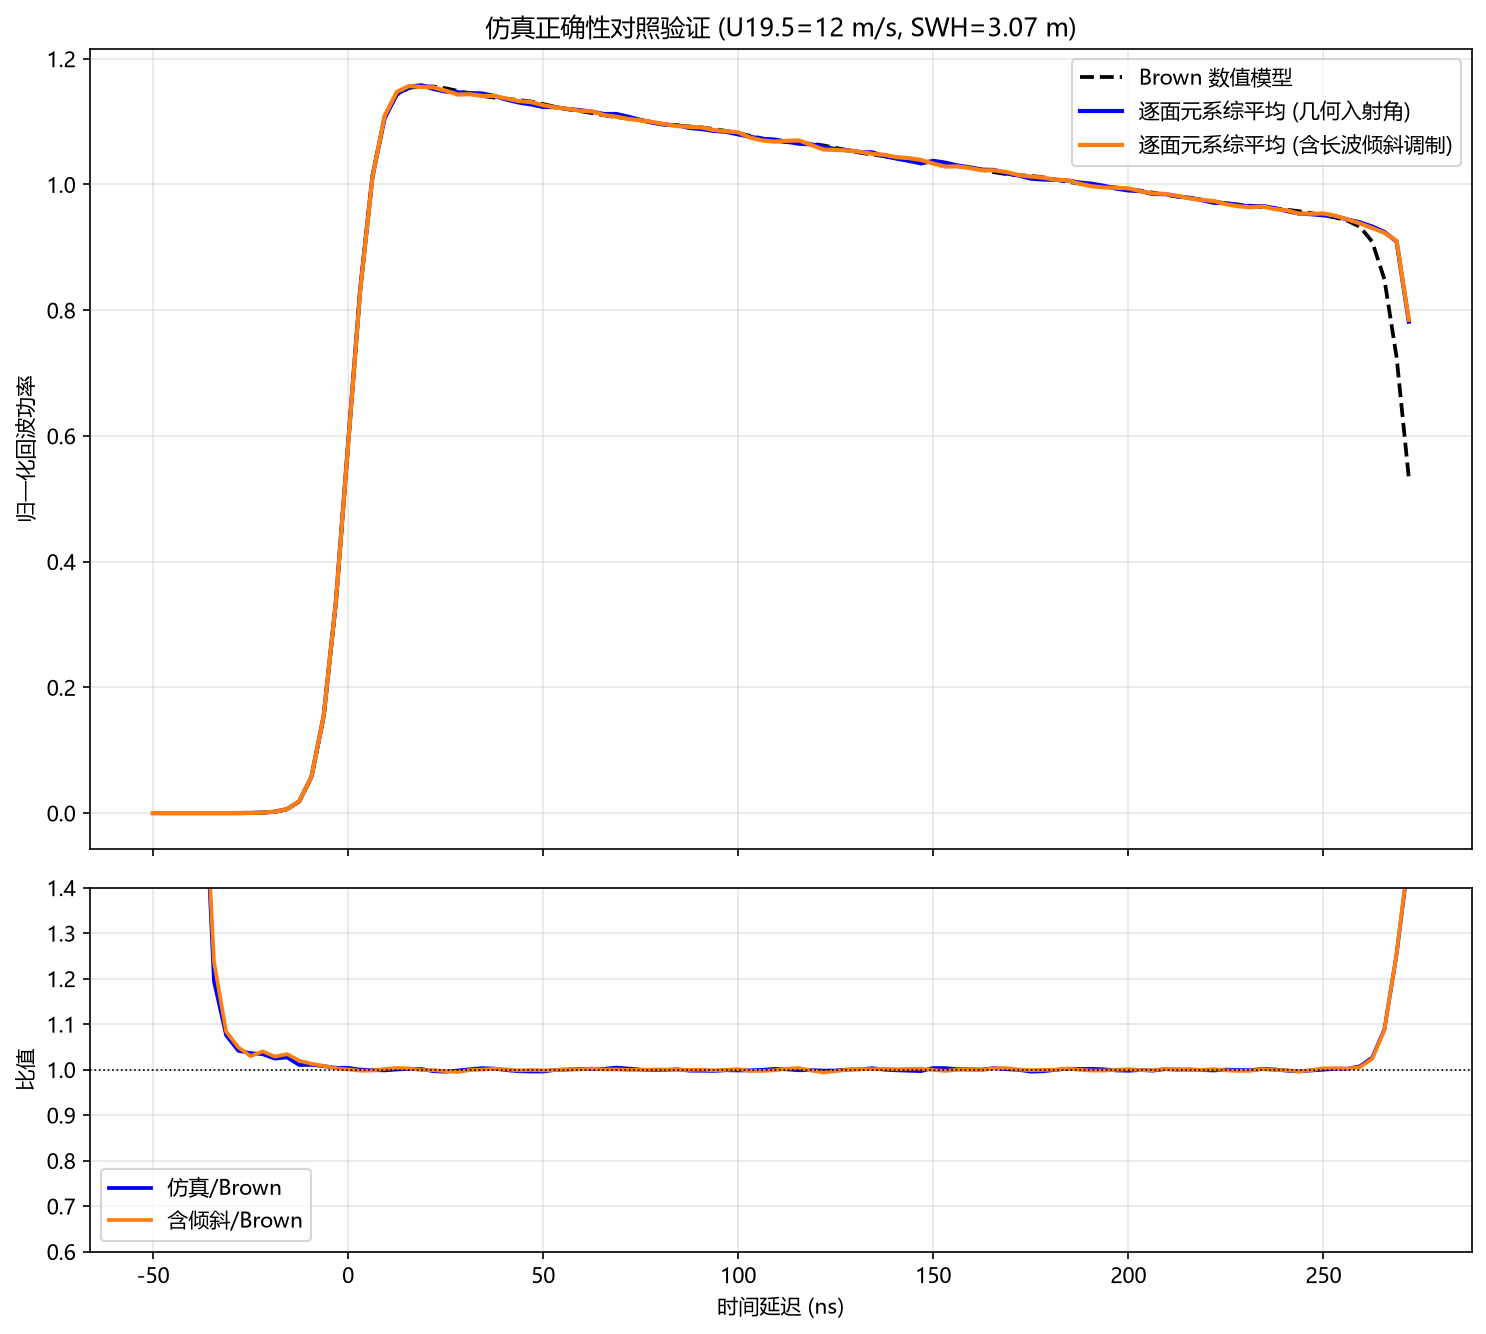
\includegraphics[width=0.7\textwidth]{validation_u12.png}
	\caption{逐面元仿真与 Brown 数值模型的对照验证（$U_{19.5} = 12$ m/s）。上：归一化平均波形；下：仿真/Brown 比值}
	\label{fig:val}
\end{figure}

\subsection{近海复合场景回波仿真}
\label{sec:coastal-sim}

近海回波畸变的根源是高度计足印内混入陆地回波。本节将三类典型陆地要素——沙滩条带、方形礁石、圆形岛屿——叠加到 PM 海面上，仿真复合场景回波，场景几何与文献\cite{refpaper}4.3 节一致。近海场景统一取 $U_{19.5} = 8$ m/s（SWH $= 1.37$ m）、系综 $M = 6$；为突出确定性的陆地特征，每组位置/占比扫描采用共同随机数（同一组海面实现，仅陆地掩膜不同）。礁石与岛屿场景的采样窗前移至 $-150$ ns 起始，以容纳海拔引起的回波提前。

\subsubsection{陆地两尺度建模}

陆地微粗糙面的相关长度 $l = 1.5 \lambda \approx 3.3$ cm 远小于面元尺寸 $\mathrm{d}x = 15.6$ m，逐面元既无法也无需显式解析陆地高度场。本文对陆地采用两尺度口径：
\begin{enumerate}
	\item \textbf{面元尺度}：陆地是海拔平台，高度偏移 $\Delta h$ 只改变双程延迟（回波提前 $2 \Delta h / c$）；
	\item \textbf{微粗糙尺度}：陆地粗糙度用指数谱描述（对应文献\cite{refpaper}式(2.18)、(2.19)），其对 Ku 波段散射的贡献由截断波数 $k_c = 2\pi/\lambda$ 的指数谱斜率方差
\begin{equation}
	\sigma_s^{2} = \frac{\sigma^{2} l^{2}}{2 \pi} \left[ \int_0^{k_c} \frac{k^{2}}{1 + k^{2} l^{2}}\, \mathrm{d}k \right] \left[ \int_0^{k_c} \frac{1}{1 + k^{2} l^{2}}\, \mathrm{d}k \right]
	\label{eq:expslope}
\end{equation}
转化为各向同性 GO 散射系数
\begin{equation}
	\sigma^0_{\mathrm{land}}(\theta) = \frac{\rho_{\mathrm{land}}}{2 \pi \sigma_s^{2} \cos^{4} \theta} \exp\!\left( -\frac{\tan^{2} \theta}{2 \sigma_s^{2}} \right)
	\label{eq:landgo}
\end{equation}
\end{enumerate}

截断波数取 $k_c = 2 \pi / \lambda$：短于雷达波长的谱分量对 Ku 散射无额外贡献（两尺度截断的常规口径；若取 $\pi/\lambda$，陆地 $\sigma^0$ 约降 4 dB，不影响本文结论）。三类陆地的介质与谱参数列于\reftab{tab:land}。沙滩与礁石微粗糙较弱（$\sigma = 0.1 \lambda$），天底 $\sigma^0$ 约 14.5--14.6 dB，\textbf{高于}同海况海面（12.5 dB）；岛屿取 $\sigma = 0.5 \lambda$，天底 $\sigma^0$ 仅 0.56 dB，\textbf{低于}海面。两类陆地与海面的强弱关系相反，恰好覆盖近海波形畸变的两种典型方向，与文献\cite{refpaper}图 4.10--4.12 的定性特征一致。

\begin{table}[htpb]
	\centering
	\caption{近海陆地要素的介质与谱参数（Ku 波段）}
	\label{tab:land}
	\song\wuhao
	\begin{tabular}{lcccccc}
		\toprule
		类型 & $\varepsilon_{\mathrm{land}}$ & $\rho_{\mathrm{land}}$ & $\sigma$ & $\sigma_s^{2}$ & $\sigma^0(0)$ (dB) & 海拔 (m) \\
		\hline
		沙滩 & $22.50 + 15.75\,\mathrm{j}$ & 0.480 & $0.1\lambda$ (2.21 mm) & $8.25 \times 10^{-3}$ & 14.64 & $+0.5$ \\
		礁石 & $22.41 + 13.87\,\mathrm{j}$ & 0.470 & $0.1\lambda$ (2.21 mm) & $8.25 \times 10^{-3}$ & 14.54 & $+2$ \\
		岛屿 & $22.41 + 13.87\,\mathrm{j}$ & 0.470 & $0.5\lambda$ (11.05 mm) & $2.06 \times 10^{-1}$ & 0.56 & $+12$ \\
		\bottomrule
	\end{tabular}
\end{table}

\hongzifuzhu{TODO：岛屿海拔 $+12$ m 为本文假设（参考论文未给出，只影响回波提前量 80 ns），导师若有口径可调。}

\subsubsection{沙滩条带占比的影响}

沙滩取 $+x$ 侧条带，面积占比 0--80\% 扫描。\reffig{fig:beach}（左）为各占比下的系综平均波形，（右）为平台窗（60--160 ns）与尾窗（220--268 ns）功率随占比的变化。结果表明\textbf{尾窗先于平台响应}：随着沙滩占比增大，足印远区（对应波形尾窗，脉冲受限环半径约 9--10 km）率先被高 $\sigma^0$ 的沙滩回波填充，尾窗功率在占比 20\% 时即显著抬升；而平台窗对应近足印，要到沙滩侵入天底附近（占比约 60\%）才明显抬升，其上限约为沙滩与海面天底 $\sigma^0$ 之差（$\approx 1.4$ dB）。“远区先变”的时序特征说明近海波形畸变往往先出现在下降沿与尾窗，为近海重跟踪的波形质量判别提供了线索。

\begin{figure}[H]
	\centering
	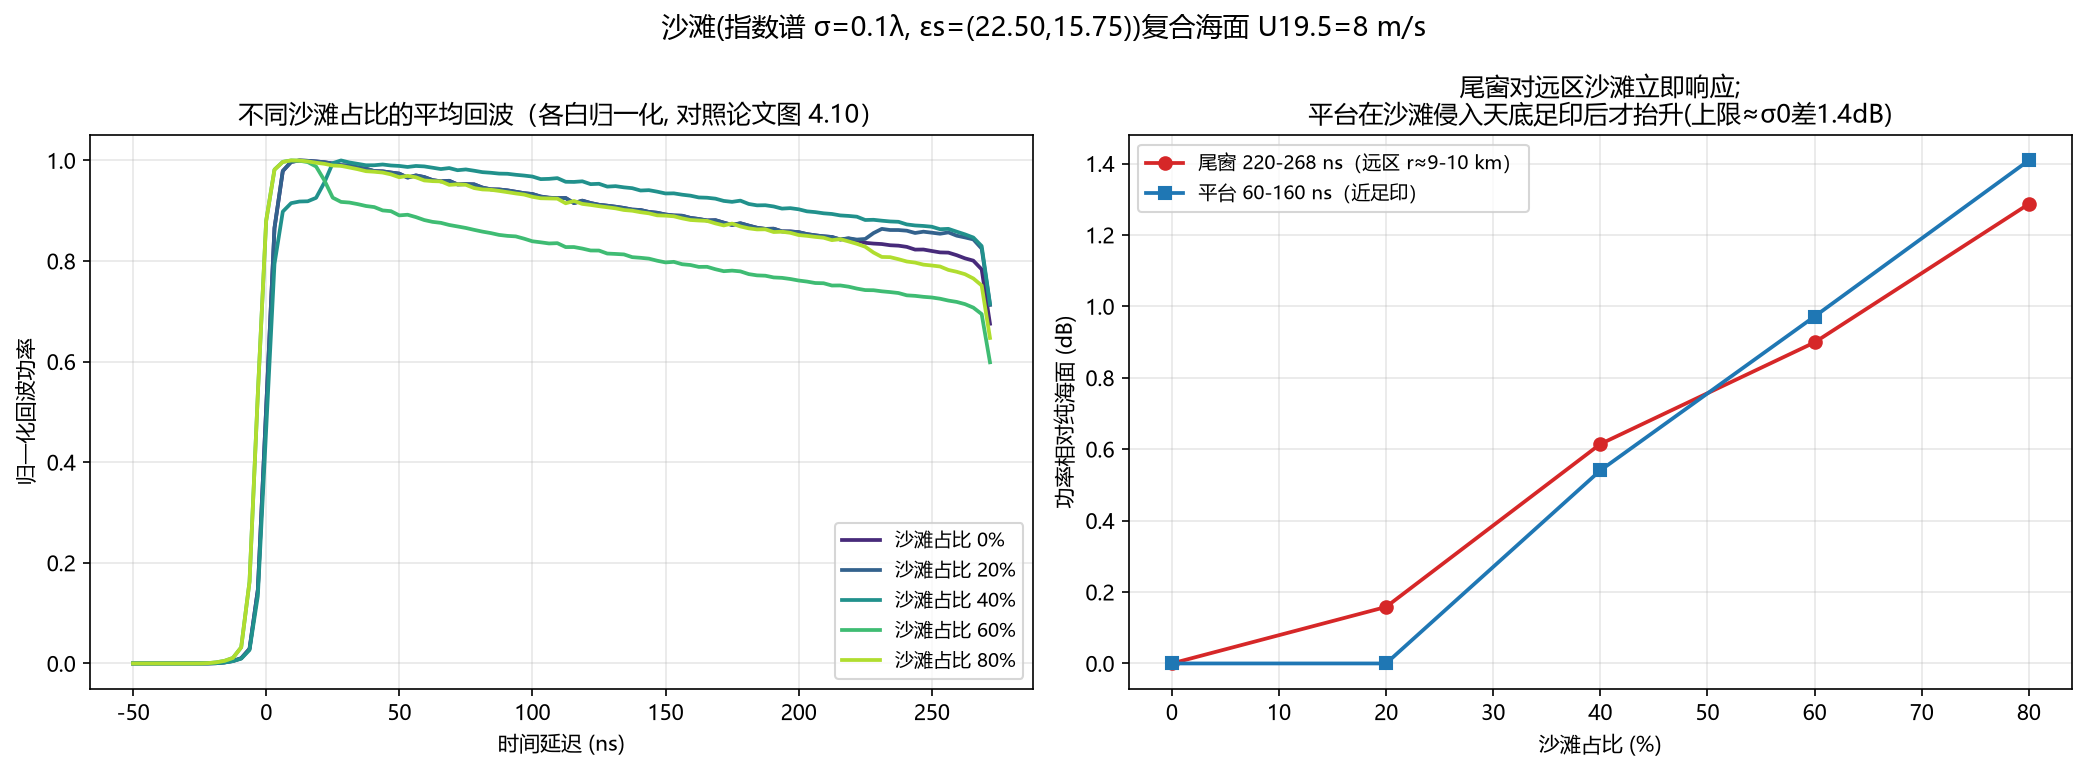
\includegraphics[width=\textwidth]{beach_fraction_scan.png}
	\caption{沙滩条带占比扫描（$U_{19.5} = 8$ m/s，$M = 6$）。左：不同占比的系综平均波形（各自归一化）；右：平台窗与尾窗功率随占比的变化}
	\label{fig:beach}
\end{figure}

\subsubsection{礁石与岛屿位置的影响}

\reffig{fig:reef} 与\reffig{fig:island} 分别给出 2 km 方形礁石（$+2$ m）与半径 1.5 km 圆形岛屿（$+12$ m）位于天底点/2.2/4.4/8.8 km（岛屿为 6.6 km）时的系综平均回波。礁石散射强于海面（$\sigma^0(0) = 14.5$ dB 对 12.5 dB），其回波因海拔 $+2$ m 整体提前 13.3 ns，在波形中形成超前于海面前沿的尖峰：位于天底点时与海面前沿重叠，抬升前沿并使前沿中点前移；随距离增大，礁石峰与海面回波在时间上逐渐分离。岛屿散射弱于海面（$\sigma^0(0) = 0.56$ dB），图中以 dB 尺度显示其弱回波：叠加在尾窗形成结构性抬升，并因海拔 $+12$ m 提前 80 ns。两类场景共同说明，近海地物的位置、海拔与粗糙度共同决定波形畸变形态，仅凭单一波形特征难以区分污染源——这正是第 \ref{chap:error} 章以拟合残差作为通用波形质量判据的动机。

\begin{figure}[htbp]
	\centering
	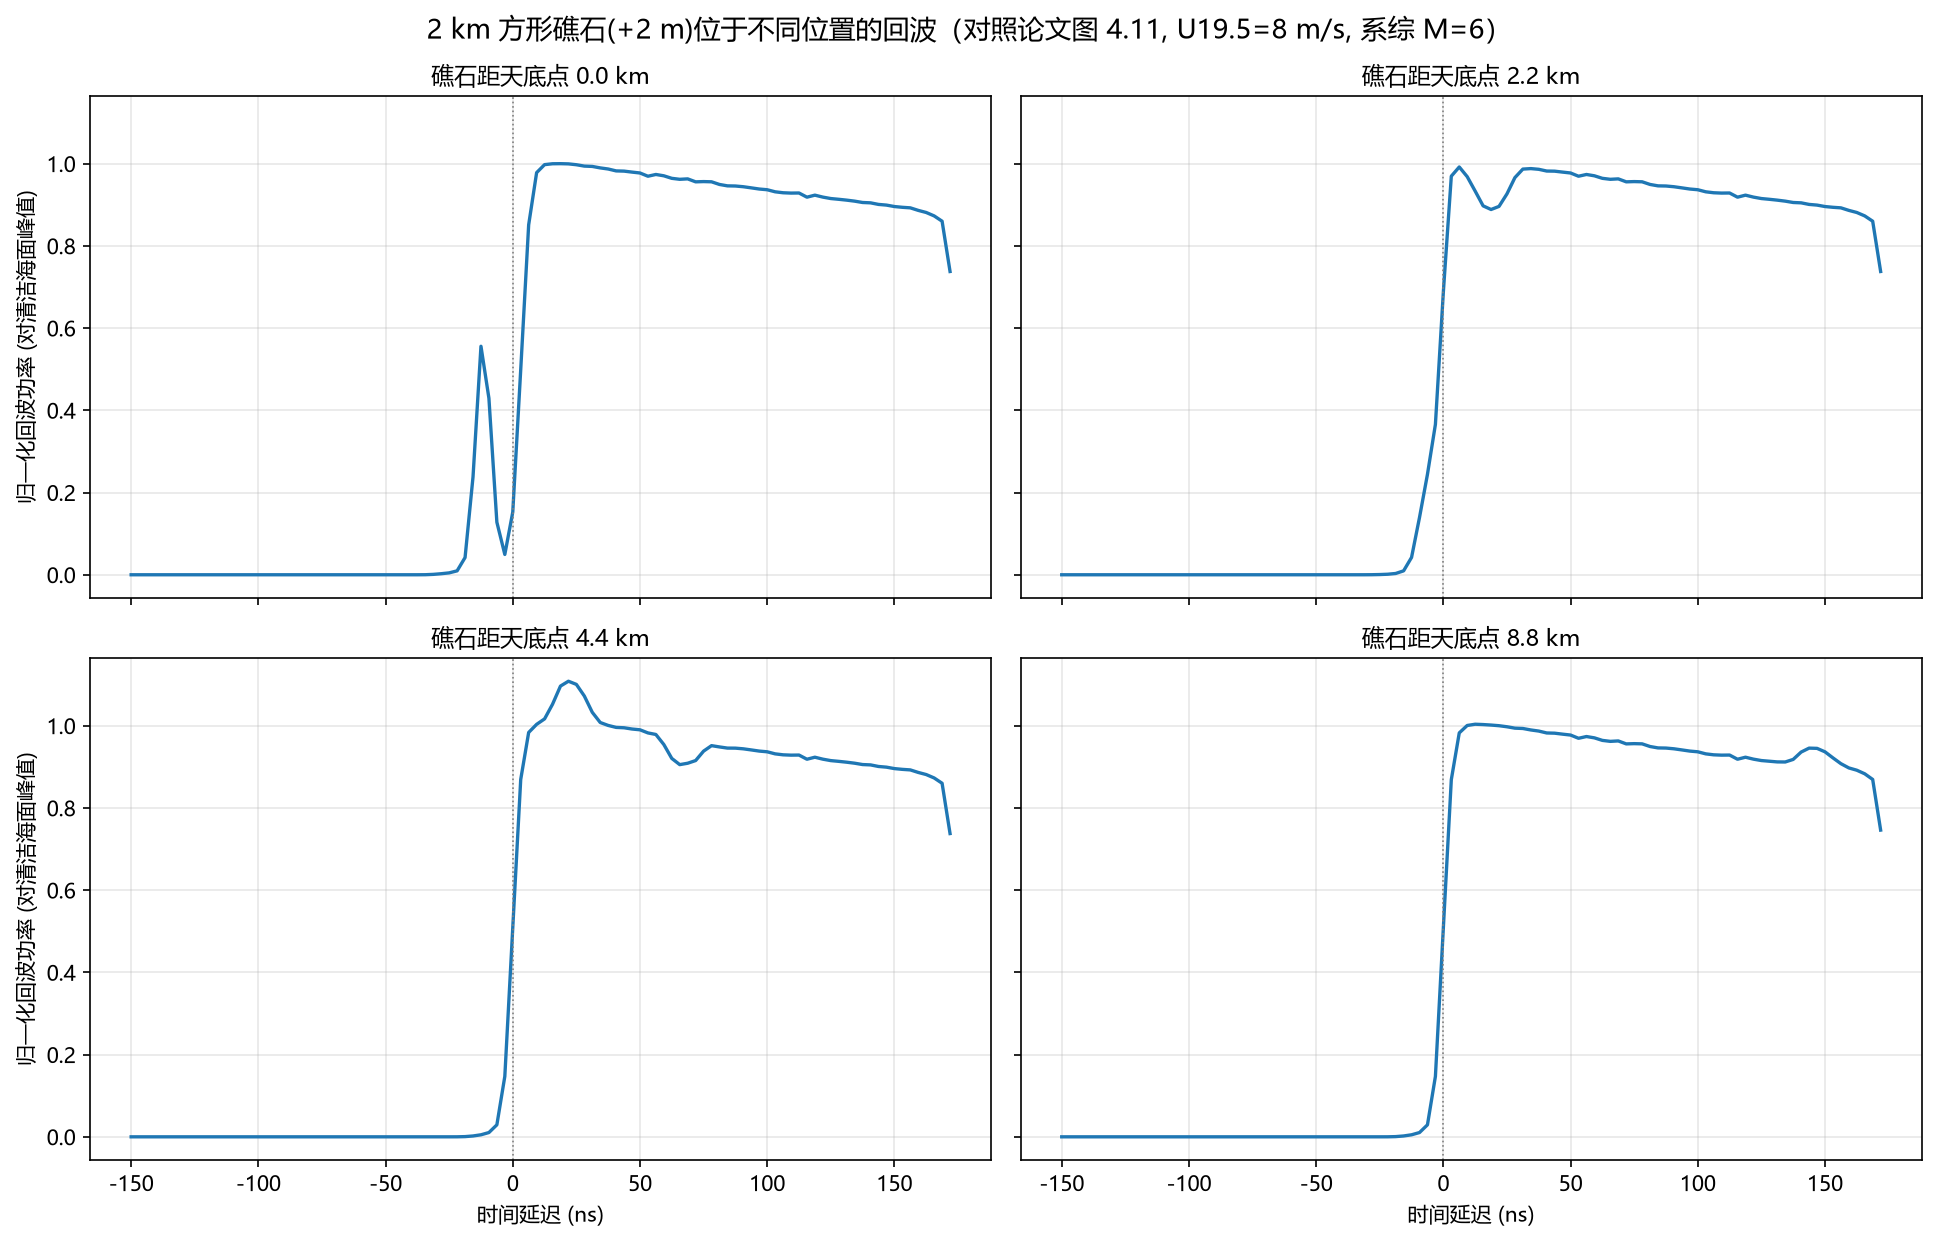
\includegraphics[width=0.9\textwidth]{reef_position_scan.png}
	\caption{2 km 方形礁石（$+2$ m）位于不同位置时的系综平均回波（相对清洁海面峰值归一化）}
	\label{fig:reef}
\end{figure}

\begin{figure}[htbp]
	\centering
	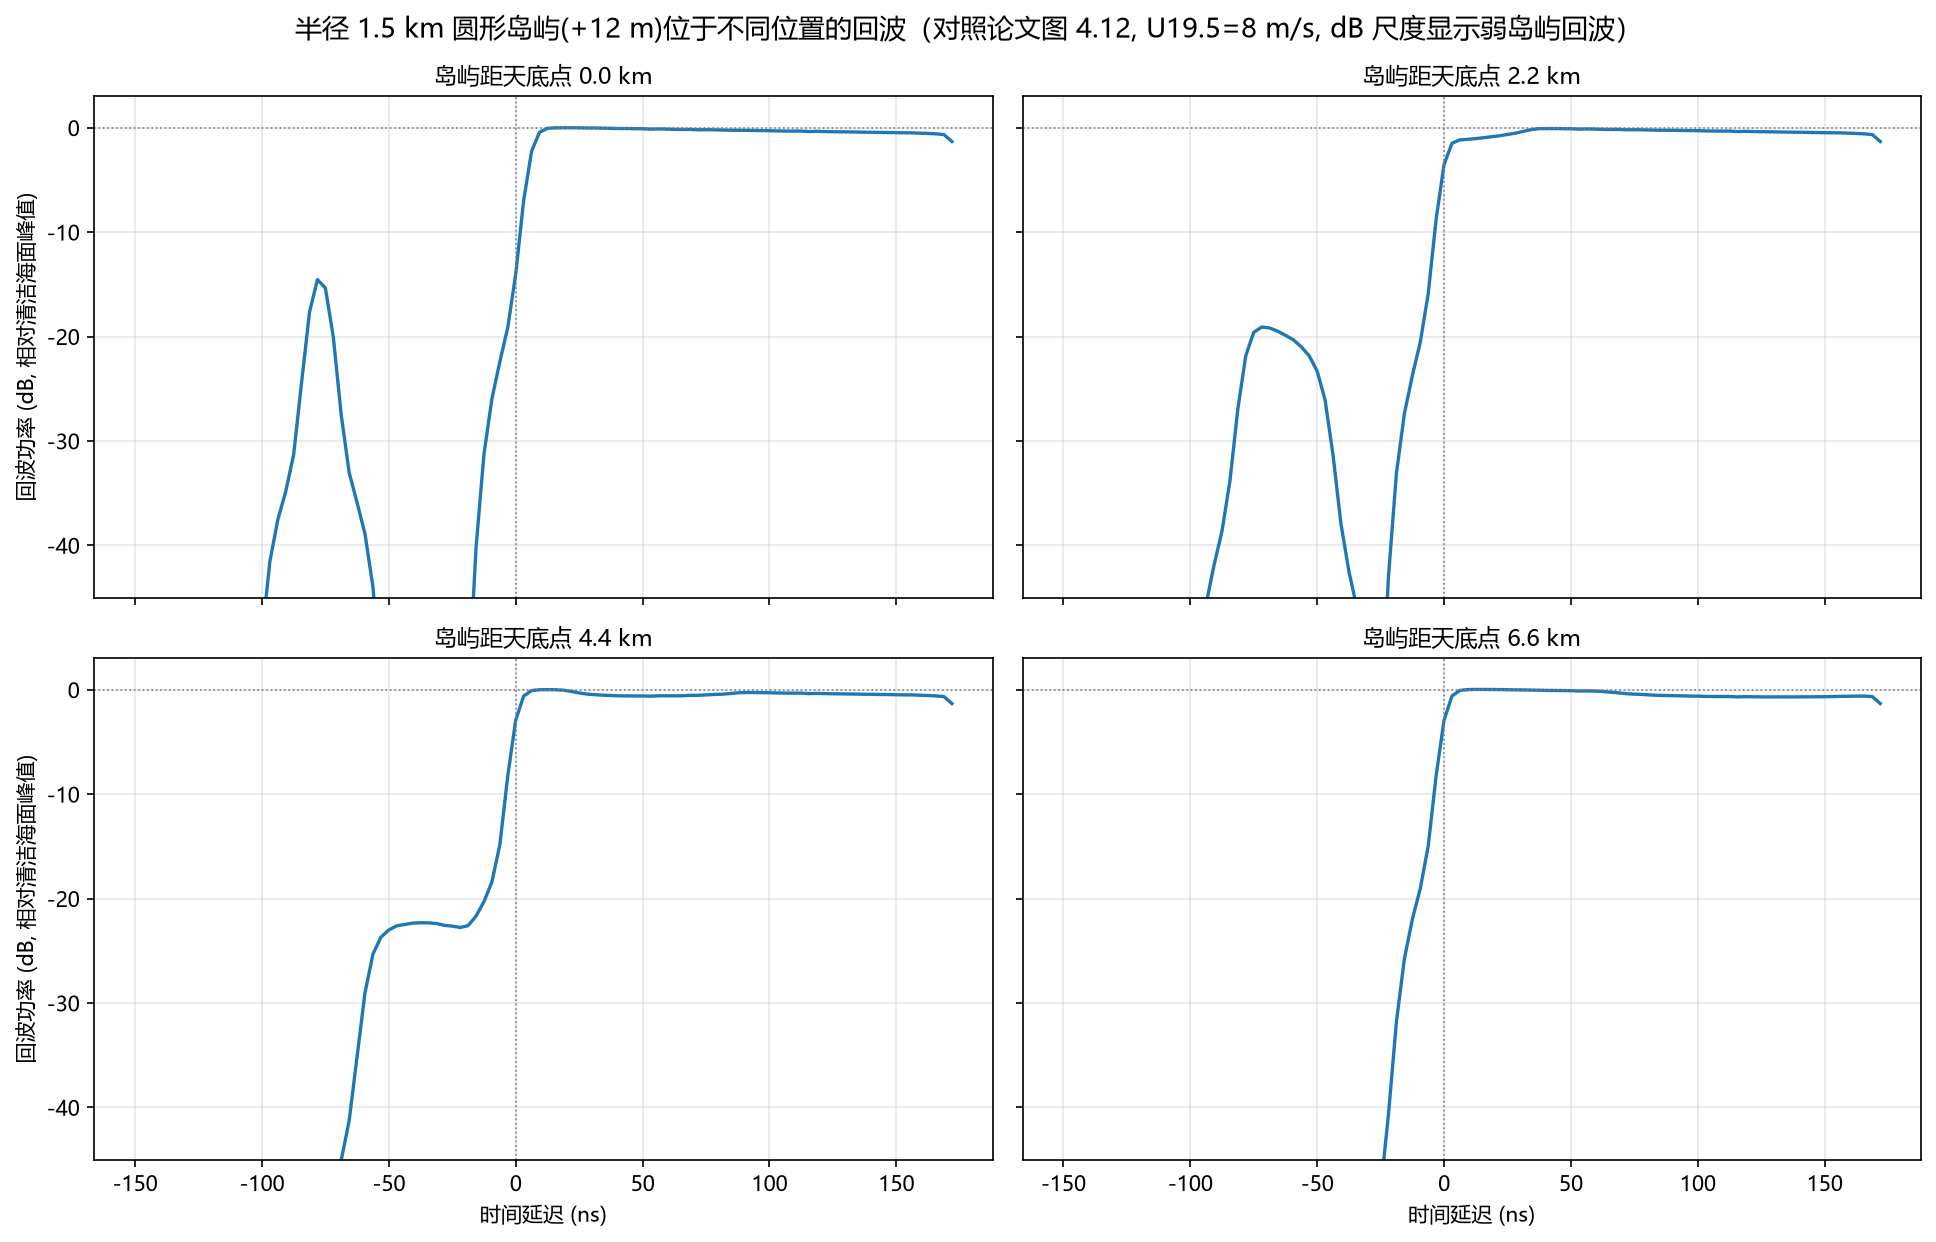
\includegraphics[width=0.9\textwidth]{island_position_scan.png}
	\caption{半径 1.5 km 圆形岛屿（$+12$ m）位于不同位置时的系综平均回波（dB 尺度）}
	\label{fig:island}
\end{figure}

\subsubsection{海水盐度与温度的敏感性}

海水相对介电常数采用 Debye 弛豫模型（Klein--Swift 型经验参数化\cite{refpaper}）：
\begin{equation}
	\varepsilon(S, T, f) = \varepsilon_\infty + \frac{\varepsilon_1(S, T) - \varepsilon_\infty}{1 + (2 \pi f \tau)^{2}} + \mathrm{j} \left[ \frac{2 \pi f \tau\, \left( \varepsilon_1(S, T) - \varepsilon_\infty \right)}{1 + (2 \pi f \tau)^{2}} + \frac{\sigma_i(S, T)}{2 \pi f \varepsilon_0} \right]
	\label{eq:debye}
\end{equation}
式中 $\varepsilon_\infty = 4.9$，静态介电常数 $\varepsilon_1$、弛豫时间 $\tau$ 与离子电导率 $\sigma_i$ 均为盐度 $S$ 与温度 $T$ 的经验多项式（具体表达式见文献\cite{refpaper}式(2.21)--(2.23)），$\varepsilon_0$ 为真空介电常数。法向菲涅尔反射率为
\begin{equation}
	\rho = \left| \frac{1 - \sqrt{\varepsilon}}{1 + \sqrt{\varepsilon}} \right|^{2}
	\label{eq:fresnel}
\end{equation}
在锚点（13.575 GHz、20 $^\circ$C、35‰）本文实现给出 $\varepsilon = (47.10,\ 39.06)$，与参考论文值 $(47.08,\ 39.07)$ 一致到第三位有效数字，对应 $\rho = 0.6173$（\reftab{tab:params}）。

由于 GO 模型中 $\sigma^0 \propto \rho$ 为纯幅度缩放，盐度与温度只平移回波平台、不改变波形形状。\reffig{fig:eps} 给出敏感性扫描：盐度 0--40‰ 引起的平台功率变化不超过 0.003 dB，完全可忽略——这正是 Ku 波段高度计反演无需盐度修正的物理依据；温度 $-2$ ~ $30\,^\circ$C 引起 $-0.20$ ~ $+0.01$ dB 的系统性变化，量级虽小但不可忽略，反演风速时需进行温度修正（其误差传播见 \ref{sec:wind} 节）。

\begin{figure}[H]
	\centering
	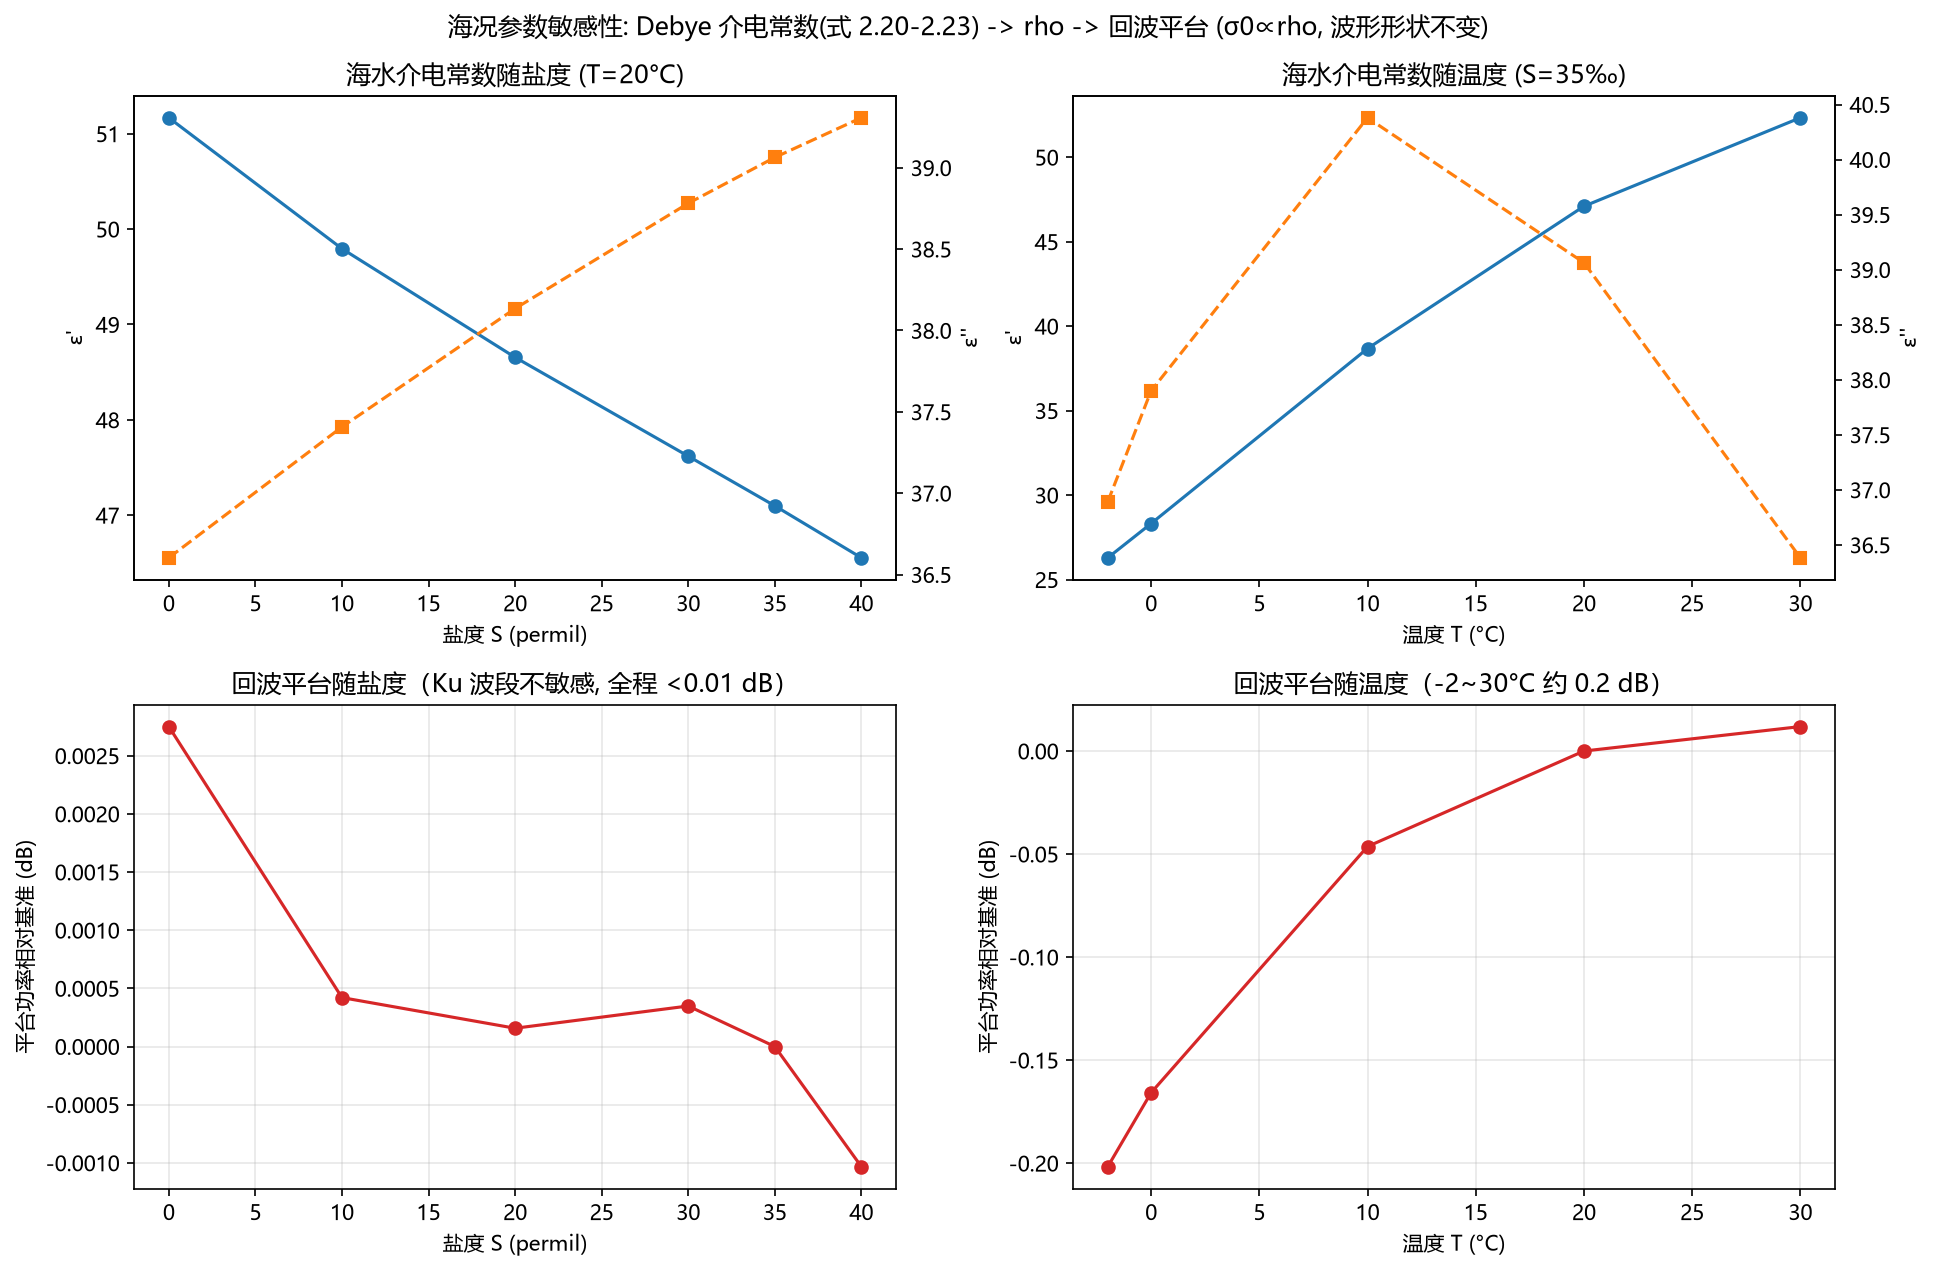
\includegraphics[width=0.9\textwidth]{salinity_temperature.png}
	\caption{海水介电常数（上排）与回波平台功率（下排）随盐度（左列，$T = 20\,^\circ$C）与温度（右列，$S = 35$‰）的敏感性}
	\label{fig:eps}
\end{figure}

综上，本章建立了“PM 谱海面 + 逐面元时域法 + 系统响应”的回波仿真链路，经 Brown 模型同口径对照验证（前沿区一致性优于 1\%），并扩展到沙滩、礁石、岛屿三类近海复合场景，定量给出了足印污染的波形畸变特征与海况参数敏感性。仿真输出的多实现波形数据（\texttt{ocean\_echo\_results.npz}、\texttt{coastal\_echo\_results.npz}）与 Jason-3 实测波形共同构成第 \ref{chap:retracking}、\ref{chap:error} 章反演与误差分析的数据基础。

\sectionbreak

% ---------------------------------------------------------------------------- %
\section{波形重跟踪与海洋参数反演方法}
\label{chap:retracking}

\subsection{反演总体流程}
\label{sec:retro-flow}
\hongzifuzhu{写什么：从 104 门波形到 SSH/SWH/U 的反演流水线总框图（预处理→初值估计→模型拟合/查表→参数输出）；SSH=t\_0·c/2、SWH=4σ\_h 的参数定义。}
\hongzifuzhu{建议配图：反演流程框图（需新画）。}

\subsection{阈值法重跟踪}
\label{sec:threshold}
\hongzifuzhu{写什么：OCOG/50\% 阈值点定位、前缘 10--90 宽度换算；系数由 Brown 模型族标定（SSH/SWH 双标定消除系统差）的做法与优点（无迭代、快、稳）。}
\hongzifuzhu{配图：fig1\_calibration.png（标定+拟合自检）。}

\subsection{Brown 数值模型最小二乘拟合}
\label{sec:brownfit}
\hongzifuzhu{写什么：数值 Brown 正向模型（平坦响应缓存）+最小二乘 (A, t\_0, σ\_h) 三参数拟合；阈值法粗估作初值；为什么误指向角 ξ 不参与联合拟合（与 (A,t\_0,σ\_c) 强耦合、不可辨识——ξ=0.3° 可被 σ\_c+1.3 ns 完全模仿；与 SGDR MLE4 不估 ξ 的工程实践一致）。}

\subsection{Hayne 二阶解析模型拟合}
\label{sec:haynefit}
\hongzifuzhu{写什么：Hayne 解析式实现；与数值 Brown 全窗 RMS 1.7\%、前沿区 <0.5\% 的一致性验证；等效误指向角扫描结论 ξ\_eq≈0。}
\hongzifuzhu{配图：fig4\_hayne\_models.png。}

\subsection{$\sigma^0$ 反演海面风速}
\label{sec:wind}
\hongzifuzhu{写什么：平台窗功率→$\sigma^0$（以 $\sigma^0$≡1 响应归一）→Cox-Munk 正演关系二分解求 U 的闭环自洽方法；盐度/温度误差传播到风速的量化（盐度 |ΔU|≤0.014 m/s 可忽略、温度 |ΔU|≤1.02 m/s 需修正）。}
\hongzifuzhu{配图：fig6\_mismatch\_wind.png（模型失配+风速闭环部分）。}

\sectionbreak

% ---------------------------------------------------------------------------- %
\section{误差分析与 Jason-3 实测数据验证}
\label{chap:error}

\subsection{误差分析总体设计}
\label{sec:error-design}
\hongzifuzhu{写什么：三层误差分析框架的定义与动机——第 1 层散斑随机误差（仿真单实现逐条反演，统计 std）、第 2 层近海畸变系统误差（污染场景 vs 各自 baseline）、第 3 层模型失配误差（长波倾斜/误指向角）；仿真数据（24 实现×3 风速+近海场景）与实测数据（Jason-3 c603p147 闽浙沿岸，2025-07-22）双数据源设计。}

\subsection{散斑随机误差与多视平均收敛}
\label{sec:speckle-error}
\hongzifuzhu{写什么：24 实现逐条反演的 SSH/SWH std（SWH 1.6--10 cm、SSH 0.2--1.1 cm）；bootstrap 平均门数实验，收敛律 ~1/√N（对应 20 Hz→1 Hz 平均）；阈值法 SWH 散斑约为拟合法 1.5 倍。}
\hongzifuzhu{配图：fig2\_speckle\_error.png。}

\subsection{近海畸变系统误差与波形质量判据}
\label{sec:nearshore-error}
\hongzifuzhu{写什么：沙滩占比/礁石/岛屿各场景的 ΔSSH/ΔSWH 偏差（礁石@天底点 +40 cm、岛屿@天底点 +78 cm、沙滩占比≥60\% 时 −53 cm）；核心发现——拟合残差 RMS 随污染激增（1.2\%→7.4\%），可作波形质量自动判据。}
\hongzifuzhu{配图：fig3\_nearshore\_bias.png。}

\subsection{模型失配误差}
\label{sec:mismatch-error}
\hongzifuzhu{写什么：长波倾斜波形用无倾斜模型反演的偏差（ΔSSH +0.25 cm / ΔSWH −0.32 cm，可忽略）；等效误指向角扫描；结论：对本文仿真口径，模型失配远小于近海畸变项。}

\subsection{Jason-3 实测数据对照验证}
\label{sec:jason3-validation}
\hongzifuzhu{写什么：数据说明（SGDR-T，cycle 603 pass 147，闽浙沿岸，2025-07-22）；开阔海（离岸>40 km）200 条 20 Hz 波形 Hayne 拟合 vs SGDR MLE4 产品：bias −0.14 m、RMS 0.77 m、相关 0.95；近海（0--10 km）拟合残差中位 10.9\% vs 开阔海 8.1\%——实测印证第 2 层“残差判据”。}
\hongzifuzhu{配图：fig5\_jason3\_validation.png；可加 Data\_Reading 的轨迹/波形图辅助。}

\subsection{误差综合讨论}
\label{sec:error-synthesis}
\hongzifuzhu{写什么：把三层误差放在一张总表/总图中对比量级，给出“近海误差预算”：散斑（随机，可平均压制）vs 近海畸变（系统，需判据剔除）vs 模型失配（本文口径可忽略）；讨论对近海高度计产品应用的启示（离岸距离多少 km 内不可信、残差判据的工程用法）。}

\sectionbreak

% ---------------------------------------------------------------------------- %
\section{总结与展望}
\label{chap:conclusion}

\subsection{全文总结}
\hongzifuzhu{写什么：对应绪论的“主要工作”逐条总结，每条给最有代表性的量化结论。}

\subsection{不足与展望}
\hongzifuzhu{可写：低风速（U19.5<6 m/s）两尺度分解未实现；仅 Ku 波段单一频点；SAR 模式（Delay-Doppler）未涉及；实测仅一条弧段一个 cycle；ξ 联合拟合不可辨识问题的更深入研究等。}

\sectionbreak

% ------------------------------------ 致谢 ------------------------------------ %
\begin{thankpage}
	\hongzifuzhu{致谢：导师、学院/实验室、同学家人，200--300 字。}
\end{thankpage}

% ----------------------------------- 参考文献 ----------------------------------- %
\clearpage
\phantomsection
\addcontentsline{toc}{section}{参考文献}

% 方式一（推荐，成稿时用）：BibTeX
% \bibliographystyle{plain}
% \bibliography{references}

% 方式二（当前骨架占位）：手写条目
\begin{thebibliography}{99}
	\label{bibref}
	\seccontent
	\bibitem{refpaper} TODO：作者. 基于电磁散射特性的雷达高度计回波仿真与分析[D]. 武汉: 华中科技大学, 硕士学位论文.（作者与年份从参考文献/ 目录的 PDF 补齐）
	\bibitem{pm1964} Pierson W J, Moskowitz L. A proposed spectral form for fully developed wind seas based on the similarity theory of S A Kitaigorodskii. Journal of Geophysical Research, 1964, 69(24): 5181-5190
	\bibitem{thorsos1990} Thorsos E I. Acoustic scattering from a Pierson-Moskowitz sea surface. The Journal of the Acoustical Society of America, 1990, 88(1): 335-349
	\bibitem{coxmunk1954} Cox C, Munk W. Measurement of the roughness of the sea surface from photographs of the sun's glitter. Journal of the Optical Society of America, 1954, 44(11): 838-850
	\bibitem{brown1977} Brown G S. The average impulse response of a rough surface and its applications. IEEE Transactions on Antennas and Propagation, 1977, 25(1): 67-74
	\bibitem{hayne1980} Hayne G S. Radar altimeter mean return waveforms from near-normal-incidence ocean surface scattering. IEEE Transactions on Antennas and Propagation, 1980, 28(5): 687-692
	\bibitem{todo-jason3} TODO：Jason-3 / SGDR 产品文档（CNES/AVISO），绪论与第 5 章引用
	\bibitem{todo-others} TODO：绪论其余引用文献（从参考文献/ 目录整理：近海重跟踪、ALES 等）
\end{thebibliography}

% ------------------------------------ 附录 ------------------------------------ %
\clearpage
\appendix
\phantomsection
\addcontentsline{toc}{section}{附录}
\section*{附录}

\subsection*{附录 A\quad 主要符号表}
\hongzifuzhu{按出现顺序列：η(x,y)、$U_{19.5}$、$\sigma_h$、SWH、SSH、$\sigma^0$、ρ、ε、B、$t_0$、ξ 等符号与含义对照。}

\subsection*{附录 B\quad 程序清单说明}
\hongzifuzhu{三个代码模块（Data\_Reading / Echo\_Simulation / Retracking）各文件功能一览表，注明仓库地址。}

\end{document}
